\documentclass[12pt,a4paper]{book}
\usepackage[a4paper, left=2cm, right=2cm, bottom=2cm, top=2.5cm]{geometry}
\usepackage[utf8]{inputenc}
\usepackage[italian]{babel}
\usepackage{lipsum}
\usepackage{epigraph}
\usepackage{titlesec}
\newcommand{\sectionbreak}{\clearpage}





\usepackage{amsmath, amssymb, amsfonts, amsthm, fouriernc, cases}
\usepackage{microtype} %improves the spacing between words and letters

\usepackage{physics}
\usepackage{graphicx}
\usepackage{epsfig}
\usepackage{epstopdf}
\usepackage{emptypage} % no numbering in auto generated blank pages
\usepackage{enumitem} % letter in enumerate environment

%%% Store indent space for a manual use%%%
\newlength\tindent
\setlength{\tindent}{\parindent}
\renewcommand{\indent}{\hspace*{\tindent}}
%%%%%%%%%%%%%%%%%%%%%%%%%%%%%%%%%%%%%%%%%%

\usepackage{parskip} %no indentation without rapresentation ;)



\usepackage{gensymb} %degree symble


\graphicspath{{../figure/}}
\setlength{\jot}{1.5ex}



%%%%%%%%%%%%%%%%%%%%%%%%%%%%%%%%%%%%%%%%%%%%%%%%%%
%% COLOR DEFINITIONS
%%%%%%%%%%%%%%%%%%%%%%%%%%%%%%%%%%%%%%%%%%%%%%%%%%
\usepackage[svgnames]{xcolor} % Enabling mixing colors and color's call by 'svgnames'
%%%%%%%%%%%%%%%%%%%%%%%%%%%%%%%%%%%%%%%%%%%%%%%%%%
\definecolor{MyColor1}{rgb}{0.2,0.4,0.6} %mix personal color
\newcommand{\textb}{\color{Black} \usefont{OT1}{lmss}{m}{n}}
\newcommand{\blue}{\color{MyColor1} \usefont{OT1}{lmss}{m}{n}}
\newcommand{\blueb}{\color{MyColor1} \usefont{OT1}{lmss}{b}{n}}
\newcommand{\red}{\color{LightCoral} \usefont{OT1}{lmss}{m}{n}}
\newcommand{\green}{\color{Turquoise} \usefont{OT1}{lmss}{m}{n}}
%%%%%%%%%%%%%%%%%%%%%%%%%%%%%%%%%%%%%%%%%%%%%%%%%%




%%%%%%%%%%%%%%%%%%%%%%%%%%%%%%%%%%%%%%%%%%%%%%%%%%
%% FONTS AND COLORS
%%%%%%%%%%%%%%%%%%%%%%%%%%%%%%%%%%%%%%%%%%%%%%%%%%
%    SECTIONS
%%%%%%%%%%%%%%%%%%%%%%%%%%%%%%%%%%%%%%%%%%%%%%%%%%
\usepackage{titlesec}
\usepackage{sectsty}
%%%%%%%%%%%%%%%%%%%%%%%%
%set section/subsections HEADINGS font and color
\sectionfont{\color{MyColor1}}  % sets colour of sections
\subsectionfont{\color{MyColor1}}  % sets colour of sections
\subsubsectionfont{\color{MyColor1}}  % sets colour of sections

\newcommand{\rstar}{ \textcolor{red}{$\star$}}


%%%%%%%%%%%%%%%%%%%%%%%%%%%%%%%%%%%%%%%%%%%%%%%%%%
%		CAPTIONS
%%%%%%%%%%%%%%%%%%%%%%%%%%%%%%%%%%%%%%%%%%%%%%%%%%
\usepackage{caption}
\usepackage{subcaption}
%%%%%%%%%%%%%%%%%%%%%%%%
\captionsetup[figure]{labelfont={color=MyColor1}}


\makeatletter
\let\reftagform@=\tagform@
\def\tagform@#1{\maketag@@@{(\ignorespaces\textcolor{red}{#1}\unskip\@@italiccorr)}}
\renewcommand{\eqref}[1]{\textup{\reftagform@{\ref{#1}}}}
\makeatother

\usepackage[pdfencoding=auto, psdextra]{hyperref}
\usepackage{bookmark}
\hypersetup{colorlinks=true}

%%%%%%%%%%%%%%%%%%%%%%%%%%%%%%%%%%%%%%%%%%%%%%%%%%
%% Suppres Chapter sentence
%%%%%%%%%%%%%%%%%%%%%%%%%%%%%%%%%%%%%%%%%%%%%%%%%%
\titleformat{\chapter}[hang]{\bf\huge}{\thechapter}{2pc}{}



%%%%%%%%%%%%%%%%%%%%%%%%%%%%%%%%%%%%%%%%%%%%%%%%%%
%% PREPARE TITLE
%%%%%%%%%%%%%%%%%%%%%%%%%%%%%%%%%%%%%%%%%%%%%%%%%%
\title{\blue \vspace{2cm} Esercizi di Fisica \\
\blueb Scienze Agrarie / Enologia}
\author{Damiano Del Sarto, Guglielmo Lami}
\date{\today}

%%%%%%%%%%%%%%%%%%%%%%%%%%%%%%%%%%%%%%%%%%%%%%%%%%
\begin{document}
\frontmatter


\vbox{
    \centering
    \vspace{-2cm}
    \maketitle %this typesets the contents of \title, \author and \date
    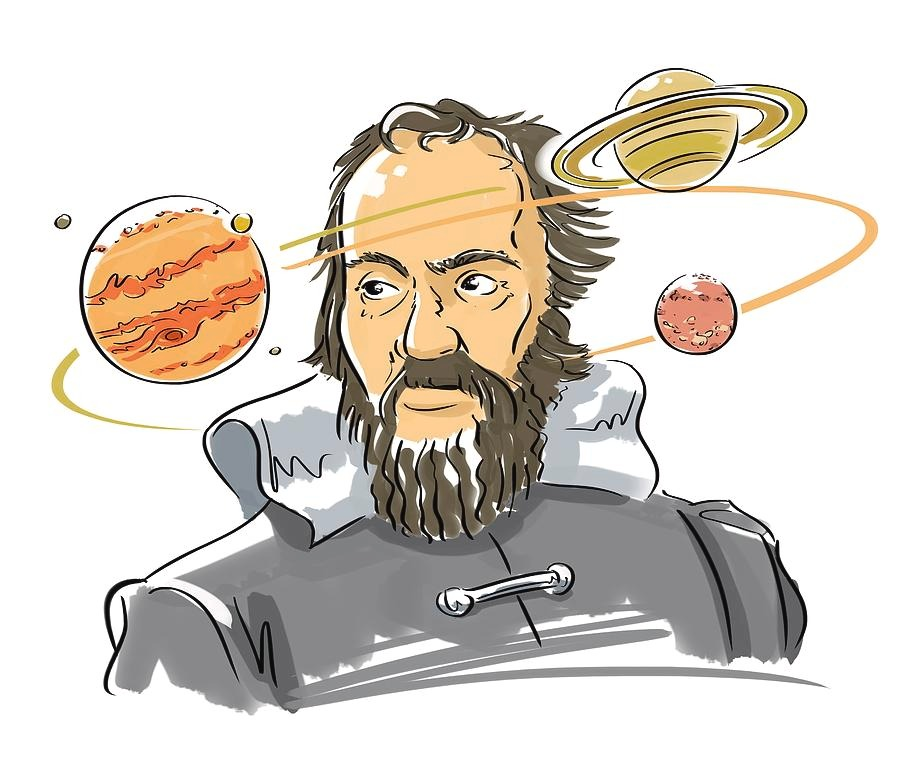
\includegraphics[scale=0.4]{Galileo.jpg}
\epigraph{"La verità riesce a imporsi solo nella misura in cui noi la imponiamo; la vittoria della ragione non può essere che la vittoria di coloro che ragionano."} {\textit{Vita di Galileo - Bertolt Brecht}}
}





\chapter{Prefazione}
\section*{Guida alla consultazione}
\addcontentsline{toc}{section}{Guida alla consultazione}
La presente raccolta ha l'obiettivo di consentire al Lettore di prendere dimestichezza coi fondamenti teorici e pratici della Fisica di base e (quindi) di superare agevolmente l'Esame di Fisica Generale per Agraria o Enologia. Un consiglio: la Fisica NON si apprende facendo esercizi. Nella Fisica ogni definizione, ogni concetto, ogni formula ha un ruolo preciso e matematicamente ben definito all'interno di una teoria coerente, con la quale è necessario avere un minimo di confidenza per poter trarre profitto dagli esercizi. In altre parole: è senza dubbio preferibile prima studiare bene la teoria e poi cimentarsi con gli esercizi. Sicuramente questi risulteranno molto più facili se avrete già chiara la struttura logica della teoria.\\

La raccolta è suddivisa in Capitoli, ognuno dei quali riguarda un macro-argomento del programma di Fisica Generale. All'interno di ogni capitolo troverete degli Esercizi e dei Problemi. I primi sono quesiti di carattere molto semplice, che richiedono la sola applicazione di concetti e formule basilari, che dovrebbero essere stati  appresi a lezione e sul libro di testo. \'E quindi indispensabile saperli risolvere senza difficoltà se si vuole superare l'esame. I Problemi invece hanno una struttura più articolata e richiedono, oltre allo Studio, logica e talvolta un pizzico di intuito. Sono catalogati in base alla difficoltà: quelli una stella sono poco più complessi degli Esercizi e corrispondono a un più che sufficiente livello di conoscenza; quelli due e tre stelle corrispondono a livelli di conoscenza buoni o addirittura ottimi e dovrebbero permettere il superamento della prova finale senza incertezze. \\

All'inizio della raccolta troverete anche un piccolo prontuario su come si affronta un esercizio di Fisica. Pensiamo che potrebbe risultare utile, specialmente per coloro che non hanno mai avuto  occasione, alle Scuole Superiori, di svolgere da soli problemi di Fisica. \\

\textbf{Buono studio e buon lavoro}!

\textit{Per errori o suggerimenti scrivete a: \href{mailto:d.delsarto2@studenti.unipi.it}{d.delsarto2@studenti.unipi.it} e \href{mailto:guglami@gmail.com}{guglami@gmail.com}
}

\newpage

\section*{Come si risolve un esercizio di Fisica}
\addcontentsline{toc}{section}{Come si risolve un esercizio di Fisica}

Quello che segue è un riferimento su come si imposta un problema di Fisica. È importante rimarcare che questo è solo un \textit{aiuto} a chi si cimenta nella talvolta ardua fatica dello svolgere problemi.

Un consiglio generale è quello di cercare sempre di capire cosa si sta facendo e non procedere a caso "rigirando" le formule: se questo approccio può funzionare su esercizi più semplici vi garantiamo che fallirà in situazioni più complesse come quelle delle prove in itinere o delle prove scritte.

Ecco dunque alcuni consigli:

\begin{enumerate}
\item \textbf{Disegnate un grafico}: nel grafico cercate di includere tutte le quantità rilevanti allo svolgimento del problema (forze, masse, distanze...). Se per problemi semplici può sembrarvi tempo sprecato, un grafico fatto \textit{bene} sarà uno devi vostri migliori alleati in problemi più articolati.
\item \textbf{Scegliete il riferimento migliore}: la scelta del sistema di riferimento spetta a voi: siete liberi di posizionare l'origine dove volete e di utilizzare coordinate cartesiane o polari. Spesso una scelta saggia del sistema di riferimento semplifica molto i calcoli.
\item \textbf{Scrivete i dati e le incognite}: per chi è alle prime armi con il calcolo letterale è facile confondere gli elementi noti da quelle che sono le incognite richieste. Farsi uno specchietto a inizio problema aiuta a non confondersi e a non perdere tempo.
\item \textbf{Risolvete i problemi in modo letterale}: oltre all'innegabile vantaggio di aver risolto un numero infinito di problemi, lasciando i dati espressi tramite un parametro (ad esempio invece di inserire il valore dell'angolo si può scrivere $\theta$), si ha un procedimento più "pulito" ed eventualmente si possono sfruttare semplificazioni algebriche (ad es. $\sin^2\theta+\cos^2\theta=1$).
\item \textbf{Controllate i casi limite}: dove possibile è interessante verificare se la descrizione che abbiamo dato del problema funziona andando a osservare alcuni casi limite. Ad esempio quando si tratta di angoli è interessate vedere cosa succede quando valgono 0° o 90°: sono spesso casi più intuitivi e una rapida verifica.
\item \textbf{Controllate le unità di misura}: nello specchietto del punto 2 è importante annotare anche le unità di misura di ogni dato in nostro possesso e delle incognite. Ad esempio se come dato ho la lunghezza $a$ del lato di un triangolo so che la sua unità di misura in KMS sarà $[a]=	\text{m}$, questo mi è utile perché, ottenuta l'espressione che identifica l'incognita cercata, posso controllare velocemente se corrisponde all'unità di misura che mi aspetto e che ho annotato nello specchietto (ad esempio per una velocità mi aspetto delle dimensioni m/s). 
\item \textbf{Controllate che le vostre equazioni abbiano senso}: non si possono sommare mele e pere! Quindi non posso sommare quantità che hanno dimensioni diverse (ad esempio metri con kg). Allo stesso modo vettori devono essere sommati con altri vettori e nelle equazioni vettoriali dovrò avere vettori al membro sinistro uguagliati a vettori al membro destro.
\item \textbf{Controllate gli argomenti di alcune funzioni}: funzioni esponenziali ($a^x$), logaritmiche ($\log(x)$) e trigonometriche ($\sin(x)$, $\cos(x)$, $\tan(x)$, $\atan(x)$, ecc...) devono avere argomento \textit{adimensionale}. Se quando eseguite il controllo dimensionale l'argomento di tali funzioni non è adimensionale avete sbagliato qualcosa.
\end{enumerate}

\tableofcontents
\thispagestyle{empty}
\newpage

\mainmatter


\chapter{Cinematica}
\section{Esercizi}

\subsection*{Esercizio 1}
Un segmento rettilineo delimitato da due punti $A$ e $B$ è lungo $\Delta x=230$ km. Un punto materiale  si muove di moto rettilineo uniforme da $A$ verso $B$.  Qual è la sua \textit{velocità scalare media} $\bar{v}$  se percorre il tratto in un tempo $\Delta t =3.25$ h? Esprimere il risultato in km/h e in m/s.
 
%\subsubsection*{Soluzione}
%Poniamo $\Delta x = 230$ km e $\Delta t = 3.25$ h. Allora, dalla definizione di velocità media ricaviamo subito:
%\begin{equation*}
%\bar{v}= \frac{\Delta x}{\Delta t}=\frac{230 \;\text{ km}}{3.25 \; \text{h}}\simeq 70.77\;  \frac{\text{ km}}{\text{h}}
%\end{equation*}\\
%Per convertire da km/h a m/s ricordiamo che $1$h=$3600$s e quindi:
%\begin{equation*}
%\frac{\text{ km}}{\text{h}}=\frac{1000 \text{ m}}{3600\text{s}}=\frac{1}{3.6}\;\frac{\text{m}}{\text{s}}
%\end{equation*}\\
%La conversione delle velocità da km/h a m/s comporta dunque una divisione per un fattore 3.6. Il risultato richiesto è dunque:\\
%\begin{equation*}
%\bar{v}\simeq \frac{70.77}{3.6} \frac{\text{m}}{\text{s}} \simeq \;   19.66 \frac{\text{m}}{\text{s}}
%\end{equation*}\\

\subsection*{Esercizio 2}
Un cavallo si allontana dal suo addestratore percorrendo in linea retta $130$ m in $14$ s. Subito dopo si gira improvvisamente e torna al galoppo verso l'addestratore, percorrendo metà della distanza in $4.8$ s. Considerando come positivo il verso della velocità del cavallo quando questi si allontana dall'addestratore
e supponendo che la velocità del cavallo sia costante in ogni tratto, determinare:
\begin{enumerate}
\item[a.]{il modulo della velocità del cavallo quando si allontana ($v_1$);}
\item[b.]{il modulo della velocità del cavallo quando torna indietro ($v_2$);}
\item[c.]{la \textit{velocità scalare media} $\bar{v}_{\text{scalare}}$ nell'intero percorso;}
\item[d.]{la \textit{velocità vettoriale media} $\bar{v}_{\text{vettoriale}}$ nell’intero percorso.}
\end{enumerate}

%\subsubsection*{Soluzione}
%Poniamo: $\Delta x_1 = 130 \;$ m, $t_1 = 14 \;$ s, $\Delta x_2 = \frac{\Delta x_1}{2}= 65 \;$ m e $t_2 = 4.8 \;$ s. \\
%\emph{a)} La velocità del cavallo nel primo tratto è data da:
%\begin{equation*}
%v_1=\frac{\Delta x_1}{t_1}= \frac{130 \; \text{m}}{14 \; \text{s}} \simeq 9.28 \frac{\text{m}}{\text{s}} 
%\end{equation*}
%\emph{b)} La velocità media del cavallo nel secondo tratto è data da:
%\begin{equation*}
%v_2=\frac{\Delta x_2}{t_2}= \frac{65 \; \text{m}}{4.8 \; \text{s}} \simeq 13.54 \frac{\text{m}}{\text{s}} 
%\end{equation*}
%\emph{c)} Per calcolare la velocità scalare media utilizziamo la definizione:
%\begin{equation*}
%\bar{v}_{\text{scalare}}=\frac{\text{spazio  totale percorso}}{\text{tempo totale trascorso}}=\frac{\Delta x_1 + \Delta x_2}{t_1 + t_2}= \frac{130 + 65}{14 + 4.8} \: \frac{\text{m}}{\text{s}}\simeq 10.37 \; \frac{\text{m}}{\text{s}}
%\end{equation*}
%\emph{d)} Per calcolare la velocità vettoriale media utilizziamo la sua definizione:
%\begin{equation*}
%\bar{v}_{\text{vettoriale}}=\frac{\text{spostamento totale}}{\text{tempo  totale  trascorso}}= \frac{\text{posizione  finale - posizione iniziale}}{\text{tempo  totale  trascorso}}	
%\end{equation*}
%e quindi:
%\begin{equation*}
%\bar{v}_{\text{vettoriale}}=\frac{\Delta x_1 - \Delta x_2}{t_1 + t_2}= \frac{130 - 65}{14 + 4.8}\frac{m}{s}\simeq 3.46 \; \frac{\text{m}}{\text{s}} 
%\end{equation*}
%Il segno $-$ è dovuto al fatto che il cavallo percorre il tratto iniziale
%con velocità positiva, mentre percorre il secondo tratto con verso opposto.\\


\subsection*{Esercizio 3}
Due locomotive si muovono su due binari rettilinei fra loro paralleli. Entrambe partono al tempo $t=0$, una dalla posizione $x=0$ e l’altra dalla posizione $x_0=8.5$ km. La prima procede ad una velocità costante di $+20$ km/h, l’altra a una velocità costante di $-30$ km/h. Dopo quanto tempo si incontreranno? In che punto si incontreranno? Esprimere i risultati rispettivamente in secondi e in km.

%\subsubsection*{Soluzione}
%Dalla teoria del moto rettilineo uniforme, sappiamo che la legge oraria di un corpo che parte da un punto $x_0$ con velocità costante $v$ è data da:\\
%\begin{equation*}
%x(t)=x_0+vt
%\end{equation*}
%Le leggi orarie delle locomotive sono quindi rispettivamente:
%\begin{gather*}
%x_1(t)=v_1 t \\
%x_2(t)=x_0 - v_2 t
%\end{gather*}
%dove $v_1=+20$ km/h e $v_2=+30$ km/h. Affinché le locomotive si incontrino deve esistere un tempo $t^*$ in cui le coordinate $x$ delle due locomotive sono uguali, ovvero:\\
%\begin{equation*}
%x_1 (t^*) = x_2(t^*) \quad \Rightarrow \quad v_1  t^* = x_0 - v_2  t^* 
%\end{equation*}
%da cui, ricavando $t^*$:\\
%\begin{equation*}
%t^* = \frac{x_0}{v_1 + v_2} = \frac{8.5}{20 +30} \; \text{h} \simeq 0.17 \; \text{h} = 0.17 \cdot 3600 \; \text{s} \simeq 612 \; \text{s}
%\end{equation*}
%Il punto $x^*$ di incontro di trova inserendo $t^*$ in una delle due leggi orarie, per esempio nella prima: 
%\begin{gather*}
%x_1(t^*)=v_1 t^*= \frac{v_1}{v_1 + v_2} x_0= \frac{2}{5}x_0=3.4 \; \text{ km}
%\end{gather*}

\subsection*{Esercizio 4}
Alcuni amici partono per un viaggio con due macchine. La prima parte al tempo $t=0$ e procede a una velocità costante di $24$ m/s; la seconda parte $100\;\text{s}$ dopo la prima. A $12$ km dal punto di partenza c’è un bivio. Quale deve essere la velocità $v_1$ della seconda macchina affinché questa raggiunga la prima macchina al bivio? Al bivio si accorgono di non aver portato la cartina e decidono di tornare insieme al punto di partenza. Percorsi 8 km in 300 s, ritrovano la cartina e si fermano. Calcolare la velocità scalare media $\bar{v}$ e la velocità vettoriale media $v_m$ di entrambe le macchine.

%\subsubsection*{Soluzione}
%\emph{a)} Calcoliamo innanzitutto quanto tempo impiega la prima macchina ad arrivare al bivio. Il tempo $t_0$ impiegato a percorrere la distanza $\Delta x_1 = 12 \; \text{km} = 1.2 \cdot 10^4 \; \text{m}$ che la separa dal bivio, procedendo alla velocità costante $v_0 = 24 \;$ m/s sarà uguale a:\\
%\begin{equation*}
%t_0 = \frac{\Delta x}{v_0}= \frac{1.2 \cdot 10^4}{24} \; \text{s} = 500 \; \text{s}
%\end{equation*}\\
%La seconda macchina parte con $\Delta t = 100 \; s$ di ritardo rispetto alla prima. Affinché le due macchine arrivino assieme, la seconda macchina dovrà perciò percorrere i $12$ km dal punto di partenza al bivio in $t_1=t_0-\Delta t = 400 \; s$. Imponendo questa condizione, ricaviamo la velocità media $v_1$ della seconda macchina:\\
%\begin{equation*}
%v_1= \frac{\Delta x_1}{t_1}=\frac{\Delta x_1}{t_0 - \Delta t}= \frac{1.2 \cdot 10^4}{400}\frac{\text{m}}{\text{s}} = 30 \; \frac{\text{m}}{\text{s}}
%\end{equation*}\\
%\emph{b)} Le due macchine percorrono $\Delta x_2=8 \;$ km$ = 8\cdot 10^3 \;$ m in $t_2=300 \;$ s, quindi la loro velocità media $v_2$ equivale a:\\
%\begin{equation*}
%v_2=\frac{\Delta x_2}{t_2}=\frac{8\cdot 10^3}{300} \: \frac{\text{m}}{\text{s}}=26.7 \: \frac{\text{m}}{\text{s}}
%\end{equation*}\\
%Possiamo allora calcolare le velocità richieste:
%\begin{itemize}
%\item{la velocità scalare media della prima macchina vale:\\
%\begin{equation*}
%\bar{v}_1 = \frac{\Delta x_1 + \Delta x_2}{t_0 + t_2}= \frac{1.2\cdot 10^4 + 8\cdot 10^3}{500 + 300} \: \frac{\text{m}}{\text{s}}= 25.00 \: \frac{\text{m}}{\text{s}}
%\end{equation*}}
%\item{la velocità scalare media della seconda macchina vale:\\
%\begin{equation*}
%\bar{v}_2 = \frac{\Delta x_1 + \Delta x_2}{t_1 + t_2}= \frac{1.2\cdot 10^4 + 8\cdot 10^3}{400 + 300} \: \frac{\text{m}}{\text{s}}\simeq 28.57 \: \frac{\text{m}}{\text{s}}
%\end{equation*}}
%\item{la velocità vettoriale media della prima macchina vale:\\
%\begin{equation*}
%v_{m1} = \frac{\Delta x_1 - \Delta x_2}{t_0 + t_2}= \frac{1.2\cdot 10^4 - 8\cdot 10^3}{500 + 300} \: \frac{\text{m}}{\text{s}}= 5.00 \: \frac{\text{m}}{\text{s}}
%\end{equation*}}
%\item{la velocità vettoriale media della prima macchina vale:\\
%\begin{equation*}
%v_{m2} = \frac{\Delta x_1 - \Delta x_2}{t_1 + t_2}= \frac{1.2\cdot 10^4 - 8\cdot 10^3}{400 + 300} \: \frac{\text{m}}{\text{s}}\simeq 5.71 \: \frac{\text{m}}{\text{s}}
%\end{equation*}}
%\end{itemize}


\subsection*{Esercizio 5}
Un aeroplano percorre $3100$ km a una velocità costante di $790$ km/h; poi incontra un vento di coda che fa aumenteare la sua velocità di $990$ km/h per i successivi $2800$ km. Qual è la durata complessiva del viaggio? Qual è la velocità scalare media dell'aeroplano in questo viaggio?

%\subsubsection*{Soluzione}
%Il tempo $\Delta t$ necessario a coprire una distanza $\Delta x$ con una velocità $v$ è ovviamente:
%\begin{equation*}
%\Delta t= \frac{\Delta x}{v}
%\end{equation*}
%quindi il nostro aereo percorrerà la prima tratta in un tempo:
%\begin{equation*}
%t_{1}=\frac{3100 \text{km}}{790 \text{km/h}}\simeq3.92\;\text{h}
%\end{equation*}
%e la seconda tratta in un tempo:
%\begin{equation*}
%t_{2}=\frac{2800 \text{km}}{(790+990) \text{km/h}}\simeq1.57 \;\text{h}
%\end{equation*} 
%La durata complessiva del viaggio è dunque $t_{tot}= t_{1}+t_{2}= 5.49 h$. Usando la definizione di velocità scalare media, troviamo:
%\begin{equation*}
%\bar{v}=\frac{\text{spazio  totale percorso}}{\text{tempo totale trascorso}}= \frac{(3100+2800) \text{km} }{5.49 \text{h}}=1075\; \frac{\text{km}}{\text{h}}
%\end{equation*}


\subsection*{Esercizio 6} 
Una palla da bowling che viaggia con velocità costante $v$ coplisce i birilli posti in fondo ad una pista da bowling lunga $16.5$ m. Il giocatore sente il rumore della palla che colpisce i birilli $2.50$ s dopo che la palla ha lasciato la sua mano. Quanto valeva $v$? Si assuma un valore della velocità del suono pari a $v_s\simeq340$ m/s.

%\subsubsection*{Soluzione}
%Possiamo pensare al suono come ad un'onda d'urto che si genera nell'istante in cui avviene lo scontro fra la palla e i birilli e che si propaga nell'aria con velocità $v_{s}\simeq340$ m/s. Il giocatore $sente$ il suono dei birilli che cadono nel momento in cui l'onda raggiunge il suo orecchio.\\
%Il tempo che trascorre tra il lancio della palla e il momento in cui il giocatore sente il botto dei birilli è dunque:
%\begin{equation}
%t_{0}=t_{palla}+t_{suono}=2.50 \; \text{s}
%\label{eq:6.1}
%\end{equation}
%dove $t_{palla}$ è il tempo necessario alla palla per percorrere tutta la pista ($\Delta x=16.5$ m) e $t_{suono}$ è il tempo necessario all'onda sonora (generata dallo scontro fra palla e birilli) per arrivare all'orecchio del giocatore (e quindi a ripercorrere nuovamente tutta la lunghezza della pista $\Delta x$). Applicando le leggi orarie possiamo scrivere:
%\begin{equation}
%t_{suono}=\frac{\Delta x}{v_s}=\frac{16.5 \text{m}}{340 \frac{\text{m}}{\text{s}}}\simeq 0.05 \; \text{s}
%\label{eq:6.2}
%\end{equation}
%e:
%\begin{equation}
%t_{palla}=\frac{\Delta x}{v_{palla}}=\frac{16.5 \text{m}}{v_{palla}}.
%\label{eq:6.3}
%\end{equation}
%Sostituendo la \ref{eq:6.2} e la \ref{eq:6.3} nella \ref{eq:6.1} otteniamo un'equazione che ha come incognita $v_{palla}$:
%\begin{equation*}
%\frac{16.5 \text{m}}{v_{palla}}+0.05 \text{s}=2.50 \; \text{s};
%\end{equation*}
%dunque:
%\begin{equation*}
%v_{palla}=\frac{16.5 \text{m}}{(2.50-0.05) \text{s}}=6.7 \; \frac{\text{m}}{\text{s}}
%\end{equation*}

\subsection*{Esercizio 7} 
Un'automobile che viaggia su un rettilineo alla velocità costante di $95\;\text{km/h}$ sorpassa una treno lungo $1.1\;\text{km}$ che va nella stessa direzione su un binario parallelo alla strada. Se la velocità del treno è costante e pari a $75\;\text{km/h}$, quanto tempo impiegherà l'auto a superarlo e quale distanza avrà percorso in questo intervallo di tempo? Come cambiano i risultati se il treno viaggia con la velocità in modulo uguale a prima ma con verso opposto rispetto a quella dell'auto?

%\subsubsection*{Soluzione}
%Scriviamo le leggi orarie per l'automobile $x_{\text{auto}}(t)$ e per il treno $x_{\text{treno}}(t)$. Facciamo attenzione a definire le posizioni iniziali: possiamo stabilire che a $t=0$ $x_{\text{auto}}=0$ e $x_{\text{treno}}=1100\;\text{m}$. Ricaviamo quindi:
%\begin{eqnarray*}
%      x_{\text{auto}}(t)=v_{\text{auto}}t\\ 
%   x_{\text{treno}}(t)= x_{\text{treno}}(0)+v_{\text{treno}}t
%  \end{eqnarray*}
%Imponendo: $x_{\text{auto}}(t_{\text{sorpasso}})=x_{\text{treno}}(t_{\text{sorpasso}})$ troviamo $t_{sorpasso}$, ovvero il tempo necessario all'auto per superare il treno:
%\begin{equation*}
%t_{\text{sorpasso}}=\frac{x_{\text{treno}}(0)}{v_{\text{auto}}-v_{\text{treno}}}=\frac{1100 \;\text{m}}{5.5\;\text{m/s}}=200\;\text{s}
%\end{equation*}
%In questo tempo l'auto avrà percorso uno spazio pari a:
%\begin{equation*}
%x_{\text{auto}}(t_{\text{sorpasso}})=v_{\text{auto}}t_{\text{sorpasso}}=5.3 \; \text{km}
%\end{equation*}
%Se il treno avesse avuto la stessa velocità di prima ma direzione opposta al moto della macchina, ovviamente sia $t_{sorpasso}$ che $x_{\text{auto}}(t_{\text{sorpasso}})$ sarebbero stati più piccoli:
%\begin{equation*}
%t_{\text{sorpasso}}=\frac{x_{\text{treno}}(0)}{v_{\text{auto}}+v_{\text{treno}}}=\frac{1100 \text{m}}{47.22 \text{m/s}}=23.3 \;\text{s}
%\end{equation*}
%e:
%\begin{equation*}
% x_{\text{auto}}(t_{\text{sorpasso}})=v_{\text{auto}}t_{\text{sorpasso}}=615\; \text{m}
%\end{equation*}

\subsection*{Esercizio 8}
Un treno parte da una stazione da fermo e percorre, con accelerazione $a$ costante, 1.5 km in 90 s lungo un rettilineo. Quanto vale $a$? A 90 s dalla partenza, qual è la sua velocità $v$? E la velocità media $\bar{v}$ fino a quel momento?

%\subsubsection*{Soluzione}
%\emph{a)} Volendo esprimere il risultato nelle unità fondamentali poniamo $d=1.5 \; \text{km} = 1.5 \cdot 10^3 \; \text{m}$ la distanza percorsa dal treno in $t^*=90 \; \text{s}$ e calcoliamo quale deve essere la sua accelerazione affinché ciò avvenga. Partendo dalla legge oraria per il moto uniformemente accelerato, imponiamo:\\
%\begin{equation*}
%d=x_0+v_0 t^* + \frac{1}{2}a (t^*)^2 = \frac{1}{2} a (t^*)^2
%\end{equation*}
%Nel nostro caso, infatti, $x_0 =0$ e $v_0 = 0$, perché il treno parte da fermo e poniamo l'origine dell'asse $x$ coincidente col punto di partenza del treno. Ricaviamo $a$ dalla precedente equazione:\\
%\begin{equation*}
%a= \frac{2d}{(t^*)^2}= \frac{3 \cdot 10^3}{(90)^2} \frac{\text{m}}{\text{s}^2}\simeq 0.37 \; \frac{\text{m}}{\text{s}^2}
%\end{equation*}
%\emph{b)} Una volta nota l'accelerazione del treno, possiamo calcolare quale sia la sua velocità dopo un tempo $t^*$ dalla partenza:\\
%\begin{equation*}
%v(t^*) = v_0 + a t^* = a t^* \simeq 0.37\cdot 90 \frac{\text{m}}{\text{s}} \simeq 33.3 \; \frac{\text{m}}{\text{s}}
%\end{equation*}
%\emph{c)} Dalla definizione di velocità media, sappiamo che:\\
%\begin{equation*}
%\bar{v}= \frac{\text{spazio  percorso}}{\text{tempo  trascorso}}=\frac{d}{t^*}=\frac{1.5 \cdot 10^3}{90}\frac{\text{m}}{\text{s}}\simeq16.6\; \frac{\text{m}}{\text{s}}
%\end{equation*}

\subsection*{Esercizio 9}
Un aeroplano leggero deve raggiungere una velocità di 30 m/s per poter decollare. Se la sua accelerazione è di $3 $ m/s$^2$ costante, quanto deve essere la lunghezza minima della pista per permettere il decollo?

%\subsubsection*{Soluzione}
%Cominciamo a calcolare dopo quanto tempo l'aeroplano, partendo da fermo ($v_0=0$) con accelerazione $a=3 \; \text{m/s}^2$ costante, raggiunge la velocità richiesta $V = 30 \;\text{m/s}$:
%\begin{equation*}
%V=at \Longrightarrow t=\frac{V}{a}=\frac{30}{3}\; \text{s} = 10 \; \text{s}
%\end{equation*}\\
%Quanto spazio ha percorso l'aeroplano in questo tempo? Poniamo il punto di partenza a $x_0 = 0$. Allora:\\
%\begin{equation*}
%x(t)= x_0 + v_0  t + \frac{1}{2}a t^2 = \frac{1}{2}a  t^2 = \frac{1}{2}\cdot 3 \cdot 10^2 \; \text{m} = 150 \; \text{m}
%\end{equation*}\\
%quindi la pista deve essere lunga almeno 150 m per permettere all'aeroplano di decollare.\\


\subsection*{Esercizio 10}
Una macchina viaggia di moto rettilineo uniforme alla velocità di 100 km/h lungo un rettilineo. All'istante $t=0$ inizia a frenare con un'accelerazione costante di $-20\;\text{m/s}^2$  fino a fermarsi completamente. A che istante di tempo si ferma? E quanto spazio ha percorso? Ripetere i calcoli nel caso in cui la macchina abbia velocità iniziale di 200 km/h.

%\subsubsection*{Soluzione}
%Come prima cosa, conviene convertire la velocità della macchina in $m/s$:\\
%\begin{equation*}
%v_0=100 \: \frac{\text{km}}{\text{h}}= \frac{100}{3.6}\:\frac{\text{m}}{\text{s}}\simeq 27.8 \; \frac{\text{m}}{\text{s}}
%\end{equation*}\\
%A questo punto possiamo calcolare il tempo richiesto, che equivale al tempo $t$ impiegato per portare la velocità $v(t)$ da $v_0$ a $0$:\\
%\begin{equation*}
%v(t)=v_0+at=0 \Longrightarrow t= - \frac{v_0}{a}= -\frac{27.8}{-20} \: \text{s} = 1.4 \; \text{s}
%\end{equation*}\\
%In tale tempo, ponendo $x_0=0$ la posizione nel momento in cui il guidatore inizia a frenare, lo spazio percorso dalla macchina sarà:\\
%\begin{equation*}
%x(t)=x_0 + v_0 t + \frac{1}{2} a t^2 = \big(0 + 27.8 \cdot 1.4 + \frac{1}{2} \cdot (-20) \cdot (1.4)^2 \big) \: m \simeq 19.3 \; \text{m}
%\end{equation*}\\
% 
%Nel caso in cui la velocità iniziale fosse stata 200 km/h:
%\begin{equation*}
%t_{\text{frenata}}\simeq -\frac{55.5}{-20}\text{s}\simeq 2.8 \; \text{s}
%\end{equation*}
%mentre
%\begin{equation*}
%x_{\text{frenata}}=(55.5\cdot 2.8-\frac{1}{2} 20\cdot (2.8)^2)\text{m}\simeq 77 \; \text{m}
%\end{equation*}
%Notiamo che raddoppiando la velocità iniziale il tempo di frenata è raddoppiato a sua volta, ma lo spazio di frenata è $quadruplicato$!

\subsection*{Esercizio 11}
Un proiettile viene sparato verticalmente \textit{verso l'alto} con velocità iniziale pari a 392 m/s. Calcolare l'altezza massima raggiunta e il tempo impiegato (accelerazione di gravità $g = 9.8 \; m/s^2$).

%\subsubsection*{Soluzione}
%Una volta sparato a velocità iniziale $v_0 = 392 \:$ m/s, il proiettile segue le leggi del moto uniformemente accelerato con accelerazione costante $g=-9.8 \:$ m/s$^2$ (il segno meno è dovuto al fatto che l'accelerazione è diretta in verso opposto alla velocità iniziale del  proiettile). Nel salire, il proiettile rallenterà sempre più fino a fermarsi, per poi cominciare a discendere. Il punto di massima altezza sarà allora quello in cui la velocità del proiettile è nulla. Calcoliamo dopo quanto tempo il proiettile si arresta:\\
%\begin{equation*}
%v(t)= v_0 + g t =0 \Longrightarrow t= -\frac{v_0}{g}= -\frac{392}{- 9.8} \: \text{s} \simeq 40 \;  \text{s}
%\end{equation*}\\
%Qual è l'altezza massima raggiunta? Possiamo ricavarla utilizzando l'equazione del moto per il proiettile, ponendo $h_0 = 0$ il punto da cui viene sparato il proiettile, e calcolando quanto valga lo spazio $h(t)$ percorso nel tempo $t$ che abbiamo appena calcolato:\\
%\begin{equation*}
%h(t) = v_0 t + \frac{1}{2}g t^2 = \left( 392 \cdot 40 - \frac{1}{2} \cdot 9.8 \cdot (40)^2 \right) \: \text{m} = 7840 \; \text{m} 
%\end{equation*}

\subsection*{Esercizio 12}
Una macchina da corsa parte da ferma, accelera per 5 secondi con un'accelerazione di 8 m/s$^2$, mantiene la velocità raggiunta per altri 5 secondi e poi frena con un'accelerazione pari a $-10 \; \text{m/s}^2$ fino a fermarsi. Quanto spazio ha percorso in tutto?

%\subsubsection*{Soluzione}
%Lo spostamento totale sarà somma di tre termini:
%\begin{itemize}
%\item{Il primo, percorso ad accelerazione costante $a_1 = 8 \; \text{m/s}^2 $ e partendo da fermo, per $\Delta t_1 = 5\;$ s;}
%\item{Il secondo, percorso a velocità costante $v_2$ (che dovremo calcolare), per $\Delta t_2 = 5\;$ s;}
%\item{Il terzo, percorso con decelerazione costante $a_2 = -10 \;\text{m/s}^2$ che dura fino a fermarsi, quindi un tempo $\Delta t_3$ che dovremo calcolare.}
%\end{itemize}
%Calcoliamo il primo tratto:\\
%\begin{equation*}
%\Delta x_1 = \frac{1}{2} a_1 (\Delta t_1)^2 = \frac{1}{2}\cdot 8 \cdot (5)^2 \; \text{m} = 100 \; \text{m}
%\end{equation*}\\
%Per calcolare il secondo contributo, dobbiamo calcolare $v_2$. Dobbiamo allora capire che velocità ha raggiunto il veicolo dopo che è trascorso $\Delta t_1$. Calcoliamo:\\
%\begin{equation*}
%v_2 = a_1 \Delta t_1 = 8 \cdot 5 \; \frac{\text{m}}{\text{s}} = 40 \;\frac{\text{m}}{\text{s}}
%\end{equation*}\\
%A questo punto siamo pronti a calcolare il secondo tratto:\\
%\begin{equation*}
%\Delta x_2 = v_2 \Delta t_2 = 40 \cdot 5 \; \text{m} = 200 \; \text{m}
%\end{equation*}\\
%
%Per il terzo contributo, è invece necessario capire in quanto tempo il veicolo, avendo velocità iniziale $v_2$, si arresta sotto l'azione di una decelerazione costante $a_3$. Imponiamo allora che dopo un certo $\Delta t_3$ dall'inizio della frenata la velocità del veicolo sia nulla:\\
%\begin{equation*}
%v(\Delta t_3) = 0 = v_2 + a_3 \cdot \Delta t_3 \Longrightarrow \Delta t_3 = - \frac{v_2}{a_3}= -\frac{40}{- 10} \; s = 4 \; \text{s}
%\end{equation*}\\
%A questo punto possiamo calcolare il terzo tratto:\\
%\begin{equation*}
%\Delta x_3 = v_2 \cdot \Delta t_3 + \frac{1}{2} \cdot a_3 \cdot (\Delta t_3)^2 = \left( 40 \cdot 4 + \frac{1}{2} \cdot (-10) \cdot (4)^2 \right) \; \text{m} = 80 \;\text{m}
%\end{equation*}\\
%
%Infine, lo spostamento totale sarà:\\
%\begin{equation*}
%\Delta x_{tot} = \Delta x_1 + \Delta x_2 + \Delta x_3 = 380 \; \text{m}
%\end{equation*}


\subsection*{Esercizio 13}  
Determinare la distanza di arresto per un'automobile con una velocità iniziale di $95$ km/h e un tempo di reazione umana di $1.0 s$: (a) per un'accelerazione $a=-4.0$ m/s$^{2}$; (b) per $a=-8.0$ m/s$^{2}$.

%\subsubsection*{Soluzione}
%La distanza di arresto è composta da due termini: $\Delta x_{tot}=\Delta x_{\text{reazione}}+\Delta x_{\text{frenata}}$. Il primo è dovuto alla distanza percorsa alla velocità costante di $95 km/h$ nel secondo di reazione del guidatore.
%\begin{equation}
%\Delta x_{\text{reazione}}=26.4 \; \frac{\text{m}}{\text{s}}\cdot 1.0 \;\text{s}=26.4 \;\text{m}.
%\end{equation}
%$\Delta x_{frenata}$ invece si ricava dalle equazioni del moto accelerato: dall'equazione
%\begin{equation*}
%v(t)=v(0)+a t,
%\end{equation*}
%imponendo $v(t_{\text{frenata}})=0$, trovo il tempo di frenata:
%\begin{equation}
%t_{\text{frenata}}=-\frac{v(0)}{a}.
%\label{eq:13.1}
%\end{equation}
%D'altra parte, possiamo dire:
%\begin{equation}
%\Delta x_{\text{frenata}}= x(t_{\text{frenata}})-x_{0}= v t_{\text{frenata}}- \frac{1}{2}a t_{\text{frenata}}^2
%\label{eq:13.2}
%\end{equation}
%e, sostituendo \ref{eq:13.1} in \ref{eq:13.2}, troviamo:
%\begin{equation}
%\Delta x_{\text{frenata}}=- v(0)\frac{v(0)}{a}+\frac{1}{2}a \left (\frac{v(0)}{a}\right )^2=-\frac{v(0)^2}{a}+\frac{1}{2}\frac{v(0)^{2}}{a}=-\frac{1}{2}\frac{v(0)^2}{a}.
%\label{eq:13.3}
%\end{equation}
%Nel caso $a=-4.0$ m/s$^2$ la \ref{eq:13.3} ci dà il risultato:
%\begin{equation*}
%\Delta x_{tot}=\Delta x_{\text{reazione}}+\Delta x_{\text{frenata}}=(26.4+87.0) m=113.4 \;\text{m}
%\end{equation*}
%mentre nel caso $a=-8.0$ m/s$^2$:
%\begin{equation*}
%\Delta x_{tot}=\Delta x_{\text{reazione}}+\Delta x_{\text{frenata}}=(26.4+43.5) \text{m}=69.9 \; \text{m}
%\end{equation*}

\subsection*{Esercizio 14}
Una lumaca si muove lungo una pista di sabbia rettilinea. La retta lungo la quale si sposta è indicata dal versore $\hat{x}$ di un sistema di riferimento cartesiano. All'istante iniziale $t_i=0$ s essa si trova nel punto $x_i=0$.  Subito dopo inizia a spostarsi e la sua velocità all'istante $t$ generico è: $\vec{v}(t)=v(t)\hat{x}$. Un naturalista si interessa del movimento della lumaca tra $t_i=0$ e $t_f=8.0\;\text{s}$ e traccia un grafico mettendo sulle ascisse il tempo $t$ (in $s$) e sulle ordinate la velocità $v(t)$ (in cm/s). Il risultato è riportato in Figura \ref{fig:lumaca}. Che tipo di moto caratterizza la lumaca nei tratti $a, b, c, d, e, f, g, h$? Qual è la massima velocità raggiunta dalla lumaca? Esprimerla in m/s e km/h. Qual è la massima accelerazione raggiunta dalla lumaca? Esprimerla in m/s$^2$ e km/h$^2$.  Sapete dire in quale punto $x_f$ si trova la lumaca a $t=t_f$? Qual è stata la sua \textit{velocità vettoriale media}? Quanta distanza ha coperto in totale?

 \begin{figure}[!ht]
 \centering
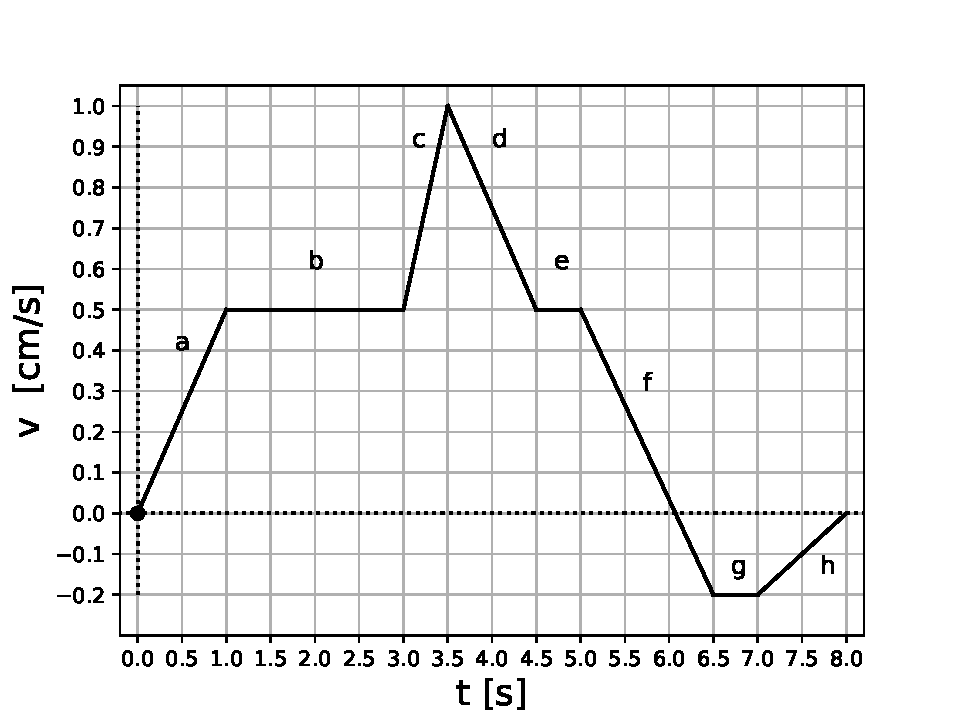
\includegraphics[scale=0.65]{lumaca.pdf}
\caption{Grafico $t$ (ascisse)/$v(t)$ (ordinate)  per il moto della lumaca oggetto dell'esercizio. \label{fig:lumaca} }
\end{figure}

%\subsubsection*{Soluzione}
%Nei tratti $b$, $e$, $g$ la velocità $v(t)$ è costante, quindi il moto è rettilineo uniforme. Nei tratti $a$, $c$, $d$, $f$, $h$ l'andamento di $v(t)$ è dato una retta, per cui $v(t)=at + \text{cost}.$ e il moto è uniformemente accelerato. (NB in effetti un moto rettilineo unifome è un moto uniformemente accelerato con $a=0$). Le accelerazioni nei tratti $a$, $c$, $d$, $f$, $h$ sono rispettivamente: 
%\begin{gather*}
%a_a=\frac{0.5 \; \text{cm/s}}{1 \; \text{s}}=0.5  \;\text{cm/s}^2 \qquad a_c=\frac{0.5 \; \text{cm/s}}{0.5 \;\; \text{s}}=1 \; \;\text{cm/s}^2 \qquad a_d=\frac{-0.5 \; \text{cm/s}}{1 \; \text{s}}=-0.5 \; \text{cm/s}^2 \\ a_f=\frac{-0.7 \; \text{cm/s}}{1.5 \; \text{s}}\simeq -0.46 \; \;\text{cm/s}^2 \qquad a_h=\frac{0.2 \; \text{cm/s}}{1 \; \text{s}}\simeq 0.2 \; \text{cm/s}^2 
%\end{gather*}
%La massima accelerazione è raggiunta quindi nel tratto $c$. Si ha: 
%\begin{gather*}
%a_c=1 \; \;\frac{\text{cm}}{\text{s}^2} = 1 \;\cdot \;\frac{10^{-2} \;\; \text{m}}{\text{s}^2}= 10^{-2} \;\frac{\text{m}}{\text{s}^2}
%\end{gather*}
%e anche (ricordando che $1$ s $= \frac{1}{3600}$ h $\simeq 2.78 \cdot 10^{-4}$ h):
%\begin{gather*}
%a_c \simeq  10^{-2} \;\cdot \;\frac{10^{-3}  \;\text{km}}{(2.78 \cdot 10^{-4}\text{h})^2} \simeq 1.29 \cdot 10^2 \; \frac{\text{km}}{\text{h}^2} 
%\end{gather*}
%La massima velocità raggiunta si legge direttamente dal grafico ed è:
%\begin{gather*}
%v^*=v \big(t=3.5 \; \text{s}\big)= 1  \;\frac{\text{cm}}{\text{s}} = 10^{-2} \;\frac{\text{m}}{\text{s}} = 3.6 \cdot 10^{-2}  \;\frac{\text{km}}{\text{h}}
%\end{gather*}
%Per calcolare la posizione finale $x_f$ occorre sommare gli spostamenti (ognuno con il giusto segno). Utilzzando le note formule del moto uniformemente accelerato si ha:
%\begin{gather*}
%\Delta x_a= \frac{1}{2} a_a \Delta t_a^2 = 0.25 \; \;\text{cm} \\
%\Delta x_b= v_b \Delta t_b = 1 \; \text{cm} \\
%\Delta x_c= \frac{1}{2} a_c \Delta t_c^2  + v_b \Delta t_c = 0.375 \; \text{cm} \\
%\Delta x_d= \frac{1}{2} a_d \Delta t_d^2  + v^* \Delta t_d = 0.75 \; \text{cm} \\
%\Delta x_e= v_e \Delta t_e = 0.25 \; \;\text{cm} \\
%\Delta x_f= \frac{1}{2} a_f \Delta t_f^2 + v_e \Delta t_f = 0.225 \;\text{cm} \\
%\Delta x_g=  v_g \Delta t_g = - 0.2 \; \;\text{cm} \\
%\Delta x_h= \frac{1}{2} a_h \Delta t_h^2 + v_g \Delta t_g = -0.1 \;\text{cm} 
%\end{gather*}
%e quindi: 
%\begin{gather*}
%x_f=x_i+\Delta x_a+\Delta x_b+\Delta x_c+\Delta x_d+ \Delta x_e+\Delta x_f=2.55\; \text{cm} 
%\end{gather*}
%Notiamo che: \textit{lo spostamento totale è uguale all'area sotto la curva $t$/$v(t)$}. Infatti ad esempio nel tratto $d$ la figura geometrica compresa tra la curva e l'asse delle ascisse è un trapezio di area: 
%\begin{gather*}
%\frac{(B+b)h}{2}=\frac{(v^*+v_e)\Delta t_d}{2}=\frac{(v^*+v^*+a_d \Delta t_d)\Delta t_d}{2}= \frac{1}{2} a_d \Delta t_d^2  + v^* \Delta t_d =\Delta x_d
%\end{gather*}
%Questo fatto è di grande importanza e ci ritorneremo. 
%La velocità vettoriale media è:
%\begin{gather*}
%\bar{v}=\frac{x_f-x_i}{t_f-t_i}\simeq 0.319  \;\frac{\text{cm}}{\text{s}}
%\end{gather*}
%La distanza totale coperta dalla lumaca si ottiene invece sommando i moduli dei $\Delta x$:
%\begin{gather*}
%d_{tot}=|\Delta x_a|+|\Delta x_b|+|\Delta x_c|+|\Delta x_d|+ |\Delta x_e|+|\Delta x_f|=3.15\;\text{cm} 
%\end{gather*}


\subsection*{Esercizio 15}
Usain Bolt e Tyson Gay partecipano alla finale dei 100 metri piani. Bolt, sin dallo sparo iniziale, mantiene una velocità costante di 36 km/h. Gay, invece, effettua un'accelerazione di 1 m/$s^2$ per tutta la durata della gara. Chi arriva prima? Con quali velocità tagliano il traguardo?

%\subsubsection*{Soluzione}
%Per capire chi dei due atleti arriva prima, dobbiamo confrontare i loro tempi di arrivo e capire chi dei due ha impiegato meno tempo. Risulta conveniente convertire la velocità di Bolt da km/h a m/s:\\
%\begin{equation*}
%v_{Bolt} = 36 \; \text{km/h} = \frac{36}{3.6} \; \text{m/s} = 10 \; \text{m/s}
%\end{equation*}\\
%Chiamiamo $x^*=100$ m il punto di arrivo della gara, e calcoliamo il tempo impiegato da ciascuno dei due atleti. Per Bolt utilizziamo l'equazione del moto rettilineo uniforme, in quanto la sua velocità è costante:\\
%\begin{equation*}
%x^*=v_{Bolt}  t_{Bolt} \Longrightarrow t_{Bolt} = \frac{x^*}{v_{Bolt}}=\frac{100 \; \text{m}}{10 \; \text{m/s}}= 10\; \text{s}
%\end{equation*}\\
%Per Gay invece è necessario utilizzare l'equazione per il moto uniformemente accelerato, in quanto lui si muove partendo da fermo (cioè $v_{Gay}(t=0)=0$) con accelerazione costante $a_{Gay} = 1 \;$ m/s$^2$:\\
%\begin{equation*}
%x^*= \frac{1}{2} a_{Gay}  t_{Gay}^2 \Longrightarrow t_{gay}= \sqrt{\frac{2x^*}{a_{Gay}}}= 14.1 \; \text{s}
%\end{equation*}\\
%quindi il vincitore è Bolt. Quali sono le loro velocità finali? Per quanto riguarda Bolt, dato che lui si muove a velocità costante, la sua velocità finale sarà sempre $v_{Bolt}= 10 \; m/s = 36 \; km/h$. Per conoscere la velocità di Gay, dobbiamo invece utilizzare l'equazione per il moto uniformemente accelerato: $v(t)= v_0 + at$. Nel caso in esame, $v_0 = 0$ perchè Gay parte da fermo. Allora, per conoscere la sua velocità finale basta sostituire nell'equazione appena vista il risultato $t_{Gay}$ appena trovato:\\
%\begin{equation*}
%v_{Gay} (t=t_{Gay})= a_{Gay} t_{Gay} = 1 \frac{m}{s^2}\cdot 14.1 \;\text{s} = 14.1 \; \text{m/s} = 50.76 \; \text{km/h}
%\end{equation*}

\subsection*{Esercizio 16}
Un vaso di fiori viene lasciato cadere da una finestra del terzo piano (10 m di altezza). Quale tempo $\Delta t$ impiega il vaso a cadere? Con che velocità arriva per terra? Se invece il vaso è stato lanciato verso il basso con una velocità di 1 m/s, come cambiano le risposte alle domande precedenti?

%\subsubsection*{Soluzione}
%\emph{a)} Nella prima parte dell'Esercizio, il vaso comincia la caduta da fermo ($v_0 = 0$) e cade per $h=10 \;$m. Poniamo l'asse verticale con origine nel punto il cui vaso comincia a cadere e verso concorde alla gravità: in questo modo $y_0=0$ e l'accelerazione di gravità $g$ è concorde all'asse, quindi positiva. Dall'equazione del moto per il moto uniformemente accelerato, posso allora calcolare quale sia il tempo $\Delta t$ che impiega il vaso a coprire la distanza $h$ imponendo:\\
%\begin{equation*}
%y(\Delta t) = h = \frac{1}{2} g\Delta t ^2 \Longrightarrow \Delta t = \sqrt{\frac{2 h}{g}}= \sqrt{\frac{2\cdot 20}{9.81}} \; \text{s} = 1.43 \; \text{s} 
%\end{equation*}\\
%La velocità con cui il vaso arriva a terra è data da:\\
%\begin{equation*}
%v(\Delta t) = v_0 + g\Delta t = g\Delta t = 9.81 \cdot 1.43 \: \frac{m}{s} = 14.02 \; \frac{m}{s}
%\end{equation*}\\

\emph{b)} Il ragionamento per questo secondo caso è identico al primo, tenendo però conto che ora $v_0 = 1 \; m/s$. Calcoliamo allora il $\Delta t_1$ in questo caso:\\
\begin{equation*}
y(\Delta t_1) = h = v_0 \Delta t_1 + \frac{1}{2} g \Delta t_1 ^2 
\end{equation*}
da cui:
\begin{equation*}
\Delta t_1 = -\frac{v_0}{g} + \sqrt{\frac{2 h}{g}+\frac{v_0^2}{g^2}}= -\frac{1}{9.81} + \sqrt{\frac{2 \cdot 10}{9.81}+\frac{1}{(9.81)^2}} \; s = 1.33 \; \text{s} 
\end{equation*}\\
Da notare che, essendo un'equazione di secondo grado in $\Delta t_1$, essa ha due soluzioni. Delle due, abbiamo però scelto l'unica che fornisce $\Delta t_1 \geq 0$.\\
Allo stesso modo del punto a), calcoliamo la velocità con cui il vaso arriva a terra:\\
\begin{equation*}
v(\Delta t_1) = v_0 + g\cdot \Delta t_1 = 1 + 9.81 \cdot 1.33 \: \frac{m}{s} = 14.04 \; \frac{m}{s}
\end{equation*}\\

\subsection*{Esercizio 17} 
Sulla Luna l'accelerazione di gravità è circa $\frac{1}{6}$ di quella sulla Terra. Se un oggetto è lanciato verso l'alto sulla Luna con velocità iniziale $v_0$, di quando arriverà più in alto rispetto ad un lancio sulla Terra con la stessa velocità iniziale?

%\subsubsection*{Soluzione}
%Se un oggetto viene lanciato verso l'alto con una velocità iniziale $v_{0}$ sulla Terra, l'altezza massima raggiunta sarà: 
%\begin{equation}
%y_{max}^{terra}=\frac{v_{0}^{2}}{2g}.
%\label{eq:17.1}
%\end{equation}
%se $g_{luna}=g/6$, sostituendo $g_{luna}$ al posto di $g$ nella \ref{eq:17.1}, troviamo:
%\begin{equation*}
%y_{max}^{luna}=\frac{v_{0}^{2}}{2g_{luna}}=\frac{6v_{0}}{2g}=6\cdot y_{max}^{terra}.
%\end{equation*}
%Quindi sulla Luna si raggiungerebbe un'altezza massima sei volte più alta che sulla Terra.

\subsection*{Esercizio 18} 
Una persona si butta in una piscina da una trampolino alto $h=4.0$ m. Il suo moto avviene esclusivamente lungo l'asse $y$.
La persona si ferma quando si trova $2.0$ m al di sotto della superficie dell'acqua. Stimate la decelerazione media della persona sotto l'acqua.

%\subsubsection*{Soluzione}
%Calcoliamo la velocità $v_{1}$ della parsona quando entra nella piscina:
%\begin{equation*}
%v_{1}=\sqrt{2gh}\simeq 8.8 \;\frac{\text{m}}{\text{s}}
%\end{equation*}
%a questo punto, sapendo che il moto del tuffatore viene frenato dopo $\Delta y=2m$ dalla superficie dell'acqua, possiamo stimare la decelerazione media supponendo che si tratti di un moto uniformememnte decelerato:
%\begin{equation*}
%a_{\text{decelerazione}}=\frac{v_{1}^2}{2\Delta y}\simeq 19\; \frac{\text{m}}{\text{s}^2}
%\end{equation*}

\newpage

\section{Problemi}
\subsection{Moto uniformemente accelerato \rstar}
Una pallina da tennis viene lanciata da terra con una velocità iniziale $\vec{v}_0$ che forma un angolo di $60^\circ$ con l'asse orizzontale, cioè con il versore $\hat{x}$. Nel sistema di riferimento cartesiano scelto l'accelerazione di gravità è $\vec{g}=-g\hat{y}$, con $g\simeq 9.81 $ m/$\text{s}^2$, e il punto di partenza della pallina è l'origine $O$ del sistema. Scrivere esplicitamente le due componenti $(v_0)_x$ e $(v_0)_y$ del vettore $\vec{v}_0$. Scrivere le due funzioni $x(t)$ e $y(t)$, ovvero la legge oraria della pallina lungo i due assi. Ricavare la traiettoria, ovvero l'equazione $y(x)$ che lega la coordinata $x$ alla 
coordinata $y$ in un generico punto del percorso tracciato dalla pallina. Trovare le coordinate del punto di massima altezza raggiunto dalla pallina. Quando la pallina si trova in questo punto, qual è il suo vettore velocità $\vec{v_1}$? E la sua accelerazione? Scrivere esplicitamente le componenti di entrambi i vettori. Calcolare la gittata del lancio, ovvero la distanza della pallina da $O$ nel momento in cui riatterra. Trovarne il valore numerico per un valore di $v$ \textit{ragionevolmente} simile alla velocità
che potreste effettivamente imprimere alla pallina lanciandola a mano.  Calcolare anche il tempo $t_f$ in cui la pallina riatterra e il vettore velocità $\vec{v_2}$ in questo istante. 

\subsubsection*{Soluzione}
Il vettore velocità iniziale è:
%
\begin{equation*}
\vec{v}_0=\big( (v_0)_x, (v_0)_y \big)= |v_0| \big( \cos (60^\circ), \sin(60^\circ)\big) = |v_0| \big(\frac{1}{2}, \frac{\sqrt{3}}{2}\big) 
\end{equation*}
%
Il moto è uniformemente accelerato lungo $\hat{y}$:
%
\begin{equation*}
y(t)=(v_0)_y t - \frac{1}{2} g t^2 = |v_0| \frac{\sqrt{3}}{2}t - \frac{1}{2} g t^2
\end{equation*}
%
Lungo $\hat{x}$ invece la pallina mantiene una velocità costante e quindi:
%
\begin{equation*}
x(t)=(v_0)_x t=|v_0| \frac{1}{2}t 
\end{equation*}
%
La traiettoria $y(x)$ lega le coordinate $x$ e $y$ e quindi si può ricavare mettendo a sistema le due ultime equazioni. Infatti se utilizziamo la seconda per ricavare: 
%
\begin{equation*}
t=\frac{2x(t)}{|v_0|}
\end{equation*}
%
sostituendo nella prima otteniamo:
%
\begin{equation*}
y(t)= |v_0| \frac{\sqrt{3}}{2} \frac{2 x(t)}{|v_0|} - \frac{1}{2} g \frac{4 x^2(t)}{|v_0|^2}
\end{equation*}
%
e quindi la traiettoria è: 
%
\begin{equation*}
y= \sqrt{3} x - \frac{2 g}{|v_0|^2} x^2
\end{equation*}
%
Si tratta di una parabola con concavità rivolta verso il basso. Il punto di massima altezza per la pallina corrisponde al vertice della parabola. Le coordinate del vertice $V$ si possono ricavare utilizzando la nota formula:
%
\begin{equation*}
y= ax^2 + bx + c \quad \Rightarrow \quad V=\big(-\frac{b}{2a}, \frac{4ac - b^2}{4a} \big)
\end{equation*}
%
(oppure semplicemente calcolando la derivata $y'(x)$ e ponendola uguale a $0$). Sostituendo $a=- \frac{2 g}{|v_0|^2}$, $b=\sqrt{3}$ e $c=0$ si ottiene: 
%
\begin{equation*}
V=\big(\frac{\sqrt{3}|v_0|^2}{4g}, \frac{3|v_0|^2}{8g}\big)
\end{equation*}
%
Detta $\vec{v_1}$ la velocità della pallina in questo punto, si avrà $(v_1)_y=0$. Infatti: se fosse $(v_1)_y>0$ allora all'istante di tempo 
successivo troveremo la pallina a una coordinata $y$ maggiore, e quindi $V$ non sarebbe il massimo in altezza della traiettoria, cosa assurda; se invece fosse $(v_1)_y<0$ allora all'istante di tempo immediatamente precedente avremmo trovato la pallina a una coordinata $y$ maggiore, di nuovo cosa assurda. La componente $(v_1)_x$ è invece uguale a $(v_0)_x=\frac{|v_0|}{2}$. Quando la pallina si trova in $V$ ha banalmente accelerazione $\vec{a}$ uguale a $\vec{g}$, come del resto in ogni punto della sua traiettoria. Il punto in cui la pallina incontra di nuovo il terreno, 
ovvero l'asse $x$, si trova uguagliando a $0$ l'espressione per
$y(x)$: 
%
\begin{equation*}
x \big(\sqrt{3}  - \frac{2 g}{|v_0|^2} x\big) =0
\end{equation*}
%
Questa equazione ha due soluzioni: $x=0$ e $x=\frac{\sqrt{3}|v_0|^2}{2g}$. La prima corrisponde all'origine $O$ cioè al punto di lancio, la seconda al punto di atterraggio. La gittata è dunque:
%
\begin{equation*}
d=\frac{\sqrt{3}|v_0|^2}{2g}
\end{equation*}
%
Notiamo che $d$ è esattamente uguale a $2$ volte la coordinata $x$ di $V$, come ci si poteva aspettare notando la simmetria della parabola rispetto all'asse verticale passante per $V$. 
Un valore ragionevole per $|v_0|$ può essere attorno a $10$ m/s. Per esempio per $|v_0|=8$ m/s si ottiene: $d\simeq 5.65$ m.
La traiettoria per questo valore è illustrata in Figura \ref{fig:traiettoria}.

 \begin{figure}[!ht]
 \centering
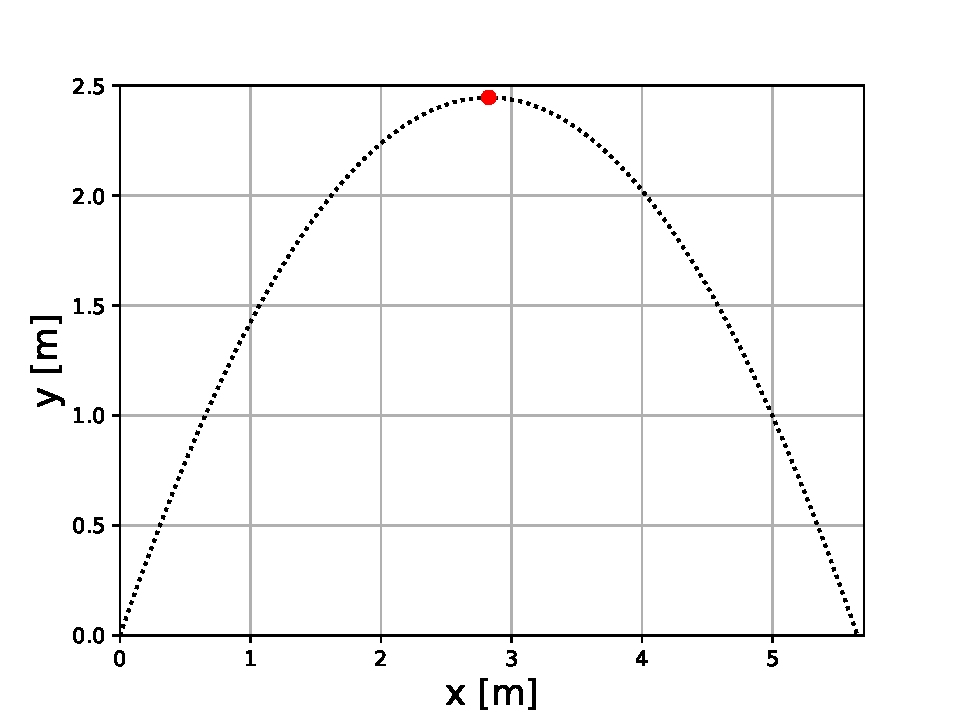
\includegraphics[scale=0.55]{traiettoria.pdf}
\caption{Traiettoria parabolica
percorsa dalla pallina ($|v_0|=8$ m/s).\label{fig:traiettoria} }
\end{figure}

Per ricavare $t_f$ basta uguagliare la gittata $d$ a $x(t_f)$:
%
\begin{equation*}
\frac{\sqrt{3}|v_0|^2}{2g}=\frac{|v_0|}{2}t_f \quad \Rightarrow \quad t_f=\frac{\sqrt{3}|v_0|}{g}
\end{equation*}
%
Le componenti di $\vec{v_1}$ saranno allora:
%
\begin{gather*}
(v_1)_x=(v_0)_x= \frac{|v_0|}{2}\\
(v_1)_y=(v_0)_y - g t_f= \frac{|v_0|\sqrt{3}}{2} - \sqrt{3}|v_0| = - \frac{|v_0|\sqrt{3}}{2}
\end{gather*}
%
Notiamo che $|\vec{v_1}|=|\vec{v_0}|$. 

\subsection{Moto uniformemente accelerato bis \rstar}
Una particella si muove su un piano cartesiano con accelerazione costante e pari a:
%
\begin{gather*}
\vec{a}=a\big(\frac{1}{\sqrt{2}},\frac{1}{\sqrt{2}}\big)
\end{gather*}
%
Che angolo forma l'accelerazione con l'asse delle $x$? Sapendo che al tempo $t_0=0$ la velocità della particella è $\vec{v_0}=(v_0,0)$ e la sua posizione $\vec{r_0}=(0,\frac{d}{2})$, scrivere la legge oraria $\vec{r}(t)$, scomponendola poi nelle due componenti. In quale istante di tempo $t_1$ la particella attraversa la retta descritta dall'equazione $y(x)=-x+2d$? Qual è il suo vettore velocità in questo istante? Che angolo forma con la velocità iniziale $\vec{v_0}$? Che angolo forma il vettore \textit{variazione di velocità} fra gli istanti $t_1$ e $t_0$ con $\vec{v_0}$? Trovare i risultati numerici per $v_0=1 \frac{\text{m}}{\text{s}}$, $d=2$ m e $a=g/4$ con $g$ l'accelerazione di gravità ($g\simeq9.81 \frac{\text{m}}{\text{s}^2}$).

\subsubsection*{Soluzione}
Il vettore $\vec{a}$ forma un angolo $\alpha=\arctan(\frac{a_y}{a_x})=\arctan(1)=\frac{\pi}{4}= 45^\circ$ con l'asse delle $x$. Il moto della particella è uniformemente accelerato e quindi la sua legge oraria si scrive: 
%
\begin{gather*}
\vec{r}(t)=\frac{1}{2}\vec{a}t^2 +\vec{v_0} t + \vec{r_0}
\end{gather*}
%
Che scomposta in componenti diventa: 
%
\begin{gather*}
x(t)=\frac{1}{2\sqrt{2}}at^2 + v_0 t \\
y(t)=\frac{1}{2\sqrt{2}}at^2  + \frac{d}{2}
\end{gather*}
%
All'istante di tempo $t_1$ in cui la particella attraversa la retta $y(x)=-x+2d$ si ha, uguagliando la coordinata y al tempo $t_1$ per la retta e per la legge oraria:
%
\begin{gather*}
y(t_1)=-x(t_1)+2d \quad \Rightarrow \quad \frac{1}{2\sqrt{2}}at_1^2  +  \frac{d}{2} = -\frac{1}{2\sqrt{2}}at_1^2 - v_0 t_1+2d
\end{gather*}
%
Si ottiene quindi un'equazione di secondo grado per $t_1$:
%
\begin{gather*}
\frac{1}{\sqrt{2}}at_1^2  + v_0 t_1 - \frac{3}{2}d =0
\end{gather*} 
%
Le due soluzioni sono:
%
\begin{gather*}
\frac{1}{\sqrt{2}a}\bigg(-v_0\pm \sqrt{v_0^2+3\sqrt{2}ad}\bigg)
\end{gather*} 
%
Solo la soluzione col $+$ è positiva, per cui è quella che ci interessa. Con i valori numerici indicati nel testo si ottiene: 
%
\begin{gather*}
t_1\simeq 1.06 \; \;\text{s}
\end{gather*} 
%
La velocità della particella a un generico istante $t$ è: 
%
\begin{gather*}
\vec{v}(t)=\vec{v}_0 + \vec{a}t
\end{gather*} 
%
che in componenti diventa:
%
\begin{gather*}
v_x(t)=v_0 + \frac{a}{\sqrt{2}}t\\
v_y(t)=\frac{a}{\sqrt{2}}t
\end{gather*} 
%
L'angolo che questo vettore forma con l'asse delle $x$, e quindi con la velocità iniziale è $\vec{v}_0$, è: 
%
\begin{gather*}
\theta=\arctan\big(\frac{\frac{a}{\sqrt{2}}t}{v_0 + \frac{a}{\sqrt{2}}t} \big)
\end{gather*} 
%
Sostituendo $t=t_1$ si trova:
%
\begin{gather*}
\theta \approx 33^\circ
\end{gather*} 
%
La variazione di velocità è $\Delta \vec{v}=\vec{v}(t)-\vec{v}_0=\vec{a}t$ o in componenti:
%
\begin{gather*}
\Delta v_x(t)=\frac{a}{\sqrt{2}}t\\
\Delta v_y(t)=\frac{a}{\sqrt{2}}t
\end{gather*} 
%
che è un vettore inclinato di $\frac{\pi}{4}=45^\circ$ rispetto all'origine. La retta, la traiettoria della particella e i vettori velocità 
$\vec{v_0}$ e $\vec{v}(t_1)$ sono rappresentati in Figura \ref{fig:particella}. 

 \begin{figure}[!ht]
 \centering
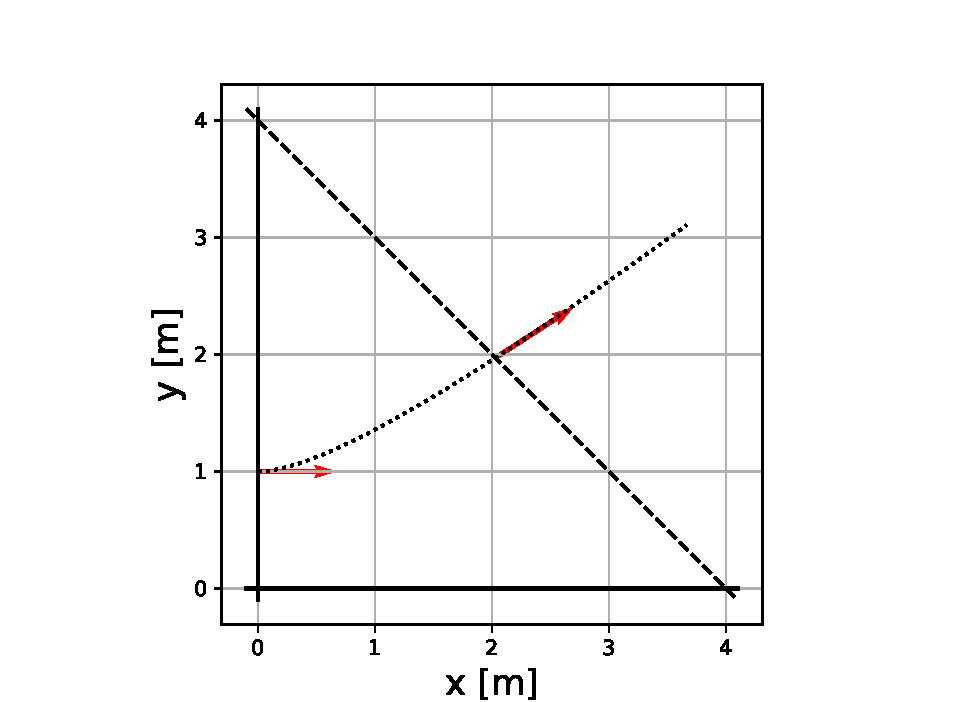
\includegraphics[scale=0.65]{particella.pdf}
\caption{Retta $y=-x+2d$, la traiettoria della particella e i vettori velocità $\vec{v_0}$ e $\vec{v}(t_1)$ (la lunghezza dei vettori in figura è puramente indicativa). I valori numerici utilizzati per $a$, $d$, $v_0$ sono quelli indicati nel testo.  \label{fig:particella} }
\end{figure}

\subsection{Lancio di un sasso \rstar}
Una pietra viene lanciata verticalmente \textit{verso l'alto}, con una velocità iniziale di $12.0$ m/s, dal bordo di uno strapiombo alto $70 $ m.
(a) Dopo quanto tempo raggiungerà la base dello strapiombo?
(b) Quale sarà la sua velocità appena prima di colpire il suolo?
(c) Quale sarà la distanza totale percorsa al momento dell'impatto?

\subsubsection*{Soluzione}
La pietra si muove di moto uniformemente accelerato lungo l'asse $y$ (nel sistema cartesiano in cui $\vec{g}=-g\hat{y}$). Detta $v_0=+12.0$ m/s la velocità iniziale della pietra, la legge oraria del corpo è:
\begin{equation*}
y(t)=h+v_0t - \frac{1}{2} gt^2 
\end{equation*}
a) Il tempo $t_f$ in cui la pietra raggiunge la base dello strapiombo
si trova imponendo che la coordinata $y$ della pietra sia $0$ al tempo $t_f$, quindi: $y(t_f)=0$. Si ha allora: 
\begin{equation*}
\frac{1}{2} gt_f^2 -v_0 t_f - h= 0 \quad \Rightarrow \quad t_f=\frac{v_0 + \sqrt{v_0^2+2hg}}{g}
\end{equation*}
Si è risolta l'equazione di secondo grado per $t_f$ prendendo l'unica soluzione fisica, quella con $t_f>0$ ovvero con il segno $+$. Inserendo i valori numerici si ottiene:
\begin{equation*}
t_f \simeq 5.19 \text{s}
\end{equation*}

b) La velocità $v_y(t)$ della pietra al tempo generico $t$ si scrive:
\begin{equation*}
v_y(t)=v_0 - gt 
\end{equation*}
La velocità un'istante prima dell'impatto a terra si ottiene ponendo $t=t_f$, con $t_f$ ricavato prima:
\begin{equation*}
v_y(t_f)=-\sqrt{v_0^2+2hg} \simeq - 39 \frac{\text{m}}{\text{s}}
\end{equation*}

c) Per trovare la distanza percorsa in totale bisogna dapprima
trovare l'altezza massima $y_{max}$ raggiunta dalla pietra. Detto $t^*$ l'istante di tempo in cui la pietra raggiunge l'altezza massima, si deve avere $v_y(t^*)=0$. Allora:
\begin{equation*}
t^*=\frac{v_0}{g} \quad \Rightarrow \quad y_{max}=y(t^*)=h+\frac{v_0^2}{g} - \frac{1}{2} \frac{v_0^2}{g} = h+\frac{1}{2} \frac{v_0^2}{g}
\end{equation*}
La distanza totale percorsa dalla pietra sarà $y_{max}-h$ (tratto in salita) \text{più} $y_{max}$ e quindi:
\begin{equation*}
d=(y_{max}-h)+y_{max}=2y_{max}- h = h+\frac{v_0^2}{g} \simeq 85 \text{m}
\end{equation*}


\subsection{Moto di un razzo \rstar}
Un razzo sale verticalmente, partendo da fermo, con un'accelerazione $a_{0}=3.2 \; \text{m/s}^2$ finché finisce il carburante a $h_{1}=1200\;\text{m}$ di altezza. Dopo questo punto, la sua accelerazione è quella di gravità, verso il basso.
\begin{enumerate}[label=\alph*)]
\item  Qual è la velocità del razzo nel momento in cui finisce il carburante?
\item Quanto tempo impiega a raggiungere quel punto?
\item Quale altezza massima raggiunge il razzo?
\item Quanto tempo occorre per raggiungere la massima altezza?
\item Con quale velocità il razzo colpisce la Terra?
\item Per quanto tempo totale il razzo rimane in aria?
\end{enumerate}


\subsubsection*{Soluzione}
I primi due punti si risolvono subito utilizzando le note leggi del moto uniformemente accelerato: 
\begin{equation*}
a) \qquad v_{1}=\sqrt{2a_{0}h_{1}}=88 \; \frac{\text{m}}{\text{s}}
\end{equation*}
\begin{equation*}
b)\qquad  t_{1}=\frac{v_{1}}{a_{0}}=27 \; \text{s}
\end{equation*}
Il tratto aggiuntivo percorso dal razzo dopo la fine del carburante, prima che la (de)celerazione $-g$ riesca a fermarlo è:
\begin{equation*}
h_{2}=\frac{v_{1}^2}{2g}=395 \;\text{m}
\end{equation*}
quindi l'altezza massima raggiunta sarà:
\begin{equation*}
c) \qquad h_{max}=h_{1}+h_{2}=1595 \; \text{m}
\end{equation*}
e il tempo impiegato per raggiungerla:
\begin{equation*}
d) \qquad t_{2}=t_{1}+\sqrt{\frac{2h_{2}}{g}}= 36 \; \text{s}
\end{equation*}
Per schiantarsi a terra il razzo dovrà poi cadere partendo dall'altezza massima (quindi con una velocità iniziale nulla) sotto l'effetto dell'accelerazione di gravità. Quindi:
\begin{equation*}
e) \qquad  v_{impatto}=-\sqrt{2gh_{max}}=-177 \; \frac{\text{m}}{\text{s}}
\end{equation*}
E infine $t_{tot}=t_{2}+t_{caduta}$, dove $t_{caduta}$ è il tempo necessario affichè il razzo si schianti a terra dopo aver raggiunto l'altezza massima:
\begin{equation*}
f)\qquad  t_{tot}=t_{2}+\sqrt{\frac{2h_{max}}{g}}=(36+18)s=54\;\text{s}.
\end{equation*}


\subsection{Attraversare un fiume \rstar\rstar}
Una barchetta, la cui velocità in acqua ferma è $v_b$, deve attraversare un fiume largo $l_y$ e risalire il fiume di $l_x$. Per fare ciò il pilota dirige la barca controcorrente con un angolo di $45\degree$. Quale è la velocità della corrente del fiume? Risolvere per: $v_b=2\;\text{m/s}$, $l_y=260\;\text{m}$, $l_x=130\;\text{m}$. La situazione è schematizzata in Figura \ref{fig:river}.

\begin{figure}[!ht]
 \centering
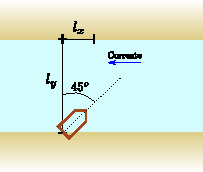
\includegraphics[scale=2]{river.pdf}
\caption{Barchetta che attraversa il fiume.  \label{fig:river} }
\end{figure}

\subsubsection*{Soluzione}
Siamo di fronte ad un problema in cui compaiono velocità relative, la relazione che lega i sistemi di riferimento è:
%
\begin{gather*}
\vec{v}=\vec{v}_{O'}+\vec{v}'
\end{gather*}
%
Per sfruttare il dato del problema sulla velocità della barchetta in acqua ferma definiamo O' il sistema di riferimento solidale con la corrente $\vec{v}_{O'}=\vec{v}_{c}$ mentre $\vec{v}'=\vec{v}_b$. Abbiamo dunque nel sistema di riferimento solidale con la sponda:
%
\begin{gather*}
\vec{v}=(-v_c+v_{bx})\hat{x}+v_{by}\hat{y}=(-v_c+\frac{\sqrt{2}}{2}v_{b})\hat{x}+\frac{\sqrt{2}}{2}v_{b}\hat{y}
\end{gather*}
%
Ora dobbiamo determinare per quanto tempo la barca naviga nel fiume, questo equivale a capire il tempo che la barca impiega per raggiungere la sponda opposta nel fiume, dunque:
%
\begin{gather*}
v_{by}=\frac{l_y}{t^*} \Rightarrow t^*=\frac{2}{\sqrt{2}}\frac{l_y}{v_b}=\sqrt{2}\frac{l_y}{v_b}
\end{gather*}
%
Adesso, conoscendo la distanza del fiume che si vuole risalire ed il tempo di percorrenza, ricaviamo quale deve essere la velocità orizzontale della corrente:
%
\begin{gather*}
l_x=(-v_c+\frac{\sqrt{2}}{2}v_{b})\cdot t^* \Rightarrow v_c=\frac{\sqrt{2}}{2}v_b -\frac{l_x}{t^*}=\frac{\sqrt{2}}{2}v_b -\frac{1}{\sqrt{2}}\frac{l_x}{l_y}v_b
\end{gather*}
%
Con i valori numerici si ottiene $v_c=\sqrt{2}/2\;\text{m/s} \approx 0.71 \;\text{m/s}$.

\subsection{Passaggio a livello \rstar}
Un uomo si trova nella sua automobile, lungo un viale rettilineo. Sulla mappa della città il viale è individuato 
dall'equazione: $y(x)=-x/\sqrt{3}$. All'istante $t_0=0$ l'uomo si trova nel punto $P=d (\frac{\sqrt{3}}{2}, -\frac{1}{2})$, con $d=500$ m. In questo stesso istante egli inizia a muoversi con accelerazione costante $a$ diretta lungo il versore $(-\frac{\sqrt{3}}{2}, +\frac{1}{2})$. Nel punto $O$ origine del sistema di riferimento cartesiano, il viale incrocia perpendicolarmente una ferrovia, anch'essa descrivibile come una retta. Scriverne l'equazione. Scrivere le componenti del vettore velocità $\vec{v}$ di un treno che si muove di moto rettilineo uniforme lungo la ferrovia, puntando nella direzione degli $x$ positivi. Supponiamo che $|\vec{v}|=100$ km/h.  Quanto vale $|\vec{v}|$ in m/s?  All'istante $t_0$ la locomotiva del treno si trova a distanza $4d$ da $O$ e ha coordinata $x$ negativa. Scrivere le coordinate della sua posizione $Q$. Se il passaggio a livello si chiude quando il treno è a distanza $2d$ dall'origine, quale dev'essere al minimo l'accelerazione $a$ dell'automobilista se egli vuole passare \textit{prima} che il passaggio a livello si chiuda? Per questo valore di $a$ scrivere le componenti del vettore velocità \textit{relativa} fra treno e automobile nell'istante in cui questa passa per $O$.
\subsubsection*{Soluzione}
Data una retta passante per l'origine $y=ax$, la retta a essa perpendicolare 
è $y=-\frac{1}{a}x$. Nel nostro caso $a=-\frac{1}{\sqrt{3}}$ e quindi
la retta che descrive la ferrovia sulla mappa della città è: $y=\sqrt{3}x$. Il versore $\hat{e}$ appartenente a questa retta e diretto verso gli $x$ positivi è: $\hat{e}=\big(\frac{1}{2}, \frac{\sqrt{3}}{2} \big)$, quindi
il vettore velocità del treno è a ogni istante:
%
\begin{equation*}
\vec{v}=|\vec{v}|\big(\frac{1}{2}, \frac{\sqrt{3}}{2} \big)
\end{equation*}
%
Si ha: 
%
\begin{equation*}
|\vec{v}|=100 \frac{\text{km}}{\text{h}}= 100 \frac{10^3 \text{  m}}{3.6 \cdot 10^3 \text{  s}}= \frac{100}{3.6} \frac{\text{m}}{\text{s}} \approx 27.78 \frac{\text{m}}{\text{s}}
\end{equation*}
%
Il punto $Q$ corrisponde a un vettore posizione diretto lungo $-\hat{e}$ e di modulo $4d$, quindi:
%
\begin{equation*}
Q=4d\big(-\frac{1}{2}, -\frac{\sqrt{3}}{2} \big)
\end{equation*}
%
La situazione è rappresentata in Figura \ref{fig:cartina}. 

 \begin{figure}[!ht]
 \centering
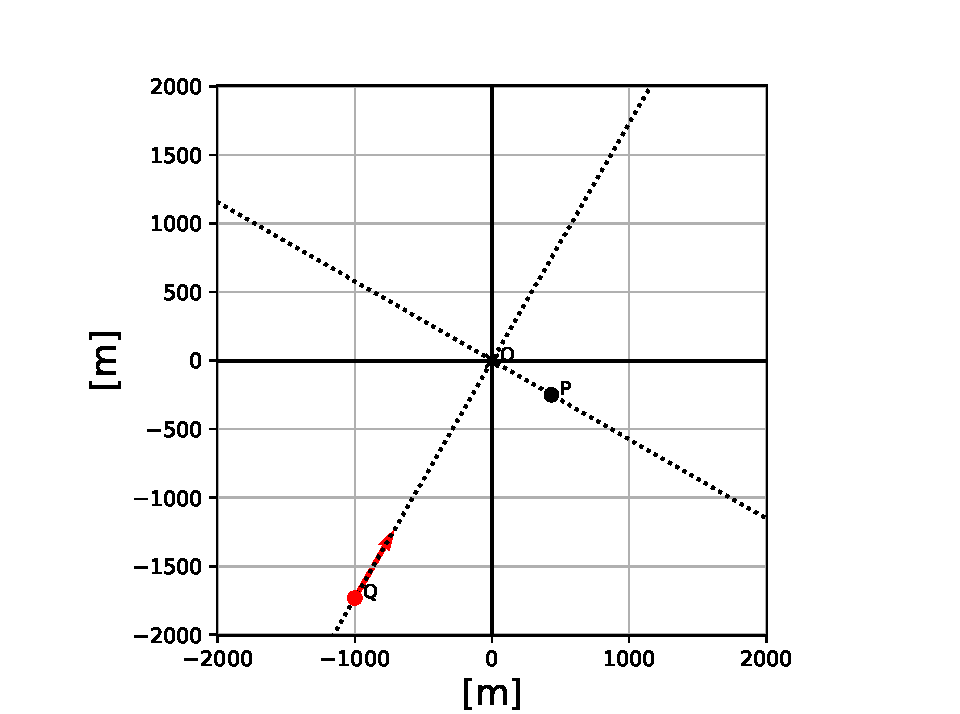
\includegraphics[scale=0.55]{cartina.pdf}
\caption{Mappa della città con la ferrovia, il viale e i punti $P$, $Q$ e $O$ (scala realistica per $d=500$ m). E' raffigurato anche il vettore velocità del treno.\label{fig:cartina} }
\end{figure}

L'automobilista si muove di moto uniformemente accelerato, con accelerazione $a$. L'istante di tempo $t_1$ in cui l'automobilista arriva a $O$ si trova ponendo $\frac{1}{2}at_1^2$ uguale allo spostamento $d$, quindi:
%
\begin{equation*}
t_1=\sqrt{\frac{2d}{a}}
\end{equation*}
%
L'istante di tempo $t_2$ in cui il treno arriva a distanza $2d$ da $O$ (cioè quando si chiude il passaggio a livello) è:
%
\begin{equation*}
t_2=\frac{2d}{|\vec{v}|}
\end{equation*}
%
La condizione che vogliamo che si realizzi è $t_2>t_1$, quindi:
%
\begin{equation*}
\frac{2d}{|\vec{v}|}>\sqrt{\frac{2d}{a}}
\end{equation*}
%
Prendendo il quadrato da entrambe le parti (N.B. si tratta di due quantità positive) si trova:
%
\begin{equation*}
a>a_{min}=\frac{|\vec{v}|^2}{2d}
\end{equation*}
%
Per i valori numerici considerati: $a_{min}\simeq 0.77$ m/s$^2$. Se $a=a_{min}$ allora nel momento in cui raggiunge $O$, l'automobile ha una velocità (in modulo):
%
\begin{equation*}
V=at_1=\frac{|\vec{v}|^2}{2d}\frac{2d}{|\vec{v}|}=|\vec{v}|
\end{equation*}
%
Il suo vettore velocità è allora:
%
\begin{equation*}
\vec{V}=|\vec{v}| \big(-\frac{\sqrt{3}}{2}, +\frac{1}{2}\big)
\end{equation*}
%
(si è considerato il versore $\big(-\frac{\sqrt{3}}{2}, +\frac{1}{2}\big)$
appartente alla retta $y(x)=-x/\sqrt{3}$).  Il vettore velocità relativa si ottiene sottraendo il vettore velocità del treno:
%
\begin{equation*}
\vec{V} - \vec{v}=|\vec{v}| \big(-\frac{\sqrt{3}}{2} - \frac{1}{2}, +\frac{1}{2} - \frac{\sqrt{3}}{2}\big)
\end{equation*}
%
\subsection{Passaggio a livello (seconda parte) \rstar\rstar}
Nella situazione dell'esercizio precedente si trovi la distanza $D$ tra la locomotiva e l'automobile ad un istante di tempo $t$ generico ($t>t_0=0$), ricavando così la funzione $D(t)$. Si determini poi a quale $t=\bar{t}$ la distanza è minima. Per facilitare i calcoli si introducano i parametri \textit{adimensionali}:
%
\begin{equation*}
f(t)=\frac{D^2(t)}{d^2}\quad \quad\alpha=\frac{a}{a_{min}}\quad \quad \tau=t\frac{v}{d}
\end{equation*}
%
e si consideri il caso particolare in cui $\alpha=2$.  \textit{Suggerimento}: si svolgano i conti nel miglior sistema di riferimento possibile...


\subsubsection*{Soluzione}
Conviene utilizzare un sistema di riferimento $S'$ che abbia come assi cartesiani i due versori:
%
\begin{equation*}
\hat{e}_1=\big(\frac{1}{2}, \frac{\sqrt{3}}{2}\big) \qquad \hat{e}_2=\big(-\frac{\sqrt{3}}{2}, \frac{1}{2}\big)
\end{equation*}
%
$S'$ si ottiene operando una rotazione di $60^\circ$ (in senso antiorario) del sistema di partenza $S$. Quindi un punto di coordinate $(x,y)$ in $S$ ha coordinate:
%
\begin{gather*}
(\frac{1}{2}x+\frac{\sqrt{3}}{2}y, -\frac{\sqrt{3}}{2}x+\frac{1}{2}y )
\end{gather*}
%
in $S'$ (Figura \ref{fig:sistema2}).  

\begin{figure}[!ht]
 \centering
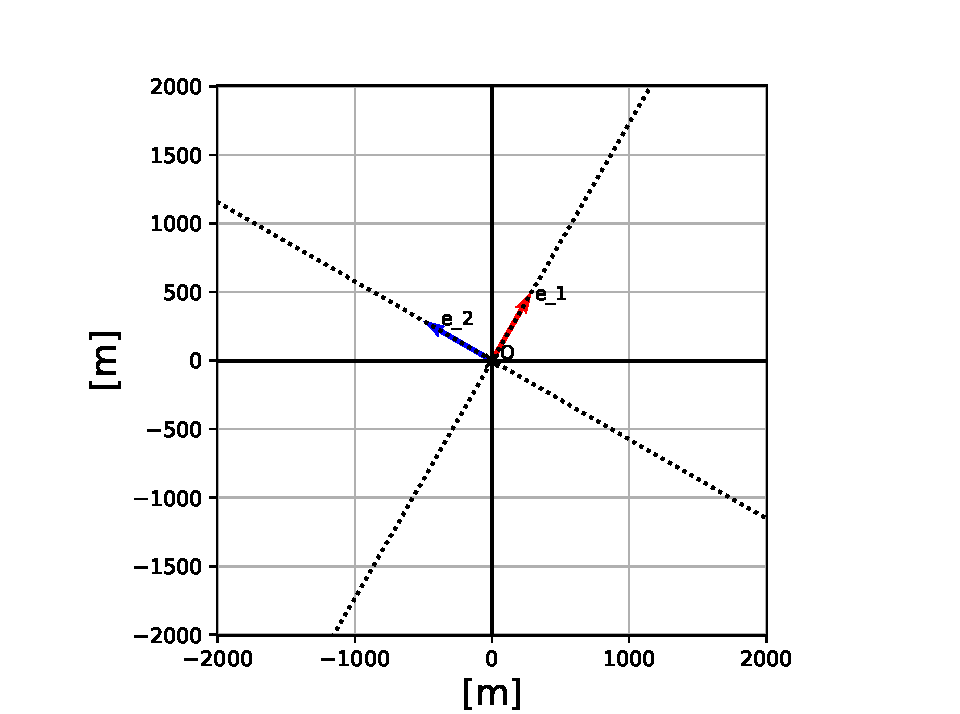
\includegraphics[scale=0.55]{sistema2.pdf}
\caption{Sistema di riferimento $S'$ dato dai versori $\hat{e}_1$ e $\hat{e}_2$. \label{fig:sistema2} }
\end{figure}


Le coordinate di $Q$ e $P$ diventano allora:
%
\begin{equation*}
Q=4d(-\frac{1}{4}-\frac{3}{4}, +\frac{\sqrt{3}}{4}-\frac{\sqrt{3}}{4})=4d(-1,0) \qquad P=d(\frac{\sqrt{3}}{4}-\frac{\sqrt{3}}{4}, -\frac{3}{4}-\frac{1}{4})=d(0,-1)
\end{equation*}
%
in $S'$, come del resto si poteva dedurre facilmente dal disegno. Le leggi orarie di treno e automobile sono allora rispettivamente:
%
\begin{gather*}
\vec{r}_T(t)=(-4d+vt,0)  \\
\vec{r}_A(t)=(0,\frac{1}{2}at^2 -d) 
\end{gather*}
%
$v$ corrisponde a $|\vec{v}|$ dell'esercizio precedente. $\vec{r}_T(t)$ e $\vec{r}_A(t)$ sono i vettori posizione 
in $S'$ a un istante generico di tempo $t>0$. La distanza tra i due oggetti è: $D(t)=|\vec{r}_T(t) - \vec{r}_A(t)|=|(-4d+vt, -\frac{1}{2}at^2 +d)|$, e quindi, ricordando la definizione di modulo di un vettore:
%
\begin{gather*}
D(t)=\sqrt{(-4d+vt)^2 + (d-\frac{1}{2}at^2)^2} =\sqrt{16d^2 -8dvt +v^2t^2 + d^2 - dat^2+\frac{1}{4}a^2t^4} = \\
=\sqrt{\frac{1}{4}a^2t^4+t^2(v^2-da)-8dvt+17d^2}\\
\end{gather*}
%
Conviene dividere tutto per $d$ ed elevare al quadrato, ottenendo così $f(t)$ come definita nel testo:
%
\begin{gather*}
f(t)=\frac{1}{4}\frac{a^2}{d^2}t^4+t^2\frac{v^2}{d^2}\big(1-\frac{ad}{v^2}\big)-8\frac{v}{d}t+17\\
\end{gather*}
%
Possiamo introdurre $a_{min}=\frac{v^2}{2d}$ dividendo e moltiplicando per questa quantità:
%
\begin{gather*}
f(t)=\frac{1}{4}\frac{a^2}{a_{min}^2}\frac{a_{min}^2}{d^2}t^4+t^2\frac{v^2}{d^2}\big(1-\frac{d}{v^2}\frac{a}{a_{min}}a_{min}\big)-8\frac{v}{d}t+17\\
\end{gather*}
%
Infine sostituendo la definizione di $a_{min}$:
%
\begin{gather*}
f(t)=\frac{1}{16}\alpha^2 \big(\frac{v}{d}t\big)^4+(1-\frac{1}{2}\alpha)\big(\frac{v}{d}t\big)^2-8\big(\frac{v}{d}t\big)+17\\
\end{gather*}
%
e quindi:
%
\begin{gather*}
f(\tau)=\frac{1}{16}\alpha^2 \tau^4+(1-\frac{1}{2}\alpha)\tau^2-8\tau+17
\end{gather*}
%
Quello che dobbiamo fare è trovare il minimo di questa funzione rispetto a $t$, oppure rispetto a $\tau$ (è la stessa cosa, sono proporzionali). Per farlo calcoliamo la derivata e imponiamola uguale a $0$:
%
\begin{gather*}
f'(\bar{\tau})=0 \quad \Rightarrow \quad \frac{1}{4}\alpha^2 \bar{\tau}^3+(2-\alpha)\bar{\tau}=8 \qquad \qquad \bar{\tau}=\bar{t}\frac{v}{d}
\end{gather*}
%
Questa è un'equazione di terzo grado, non facile da risolvere. 
Ma ponendo $\alpha=2$ come consigliato nel testo troviamo:
%
\begin{gather*}
\bar{\tau}^3=8 \quad \Rightarrow \quad  \bar{\tau}=2 \quad \Rightarrow \quad  \bar{t}=\frac{2d}{v}
\end{gather*}
%
In questo istante la distanza tra treno e automobile vale: 
%
\begin{gather*}
D(t)=\sqrt{\frac{1}{4}a^2 \frac{16d^4}{v^4}-8dv\frac{2d}{v}+17d^2}=\sqrt{4d^2-16d^2+17d^2}=\sqrt{4d^2-16d^2+17d^2}=d\sqrt{5}\\
\end{gather*}
%
In \ref{fig:distanza} sono riportati i grafici di $D(\tau)=f^2(\tau)d^2$ per differenti valori di $a$, cioè di $\alpha$ : $\alpha=0$ (linea azzurra), $\alpha=1$ (linea arancione), $\alpha=2$ (linea verde). La linea tratteggiata corrisponde a $\frac{D}{d}=\sqrt{5}$, che, come abbiamo visto, è la distanza minima per $\alpha=2$ (infatti è la tangente alla linea verde). Notare che $D(\tau=0)=D(t=0)$
è uguale in tutti i casi (perché indipendentemente da $a$ all'istante di tempo iniziale la distanza tra treno e automobile è $D(t=0)=\sqrt{(4d)^2+d^2}=d\sqrt{17}\simeq 4.12 d$).  
 \begin{figure}[!ht]
 \centering
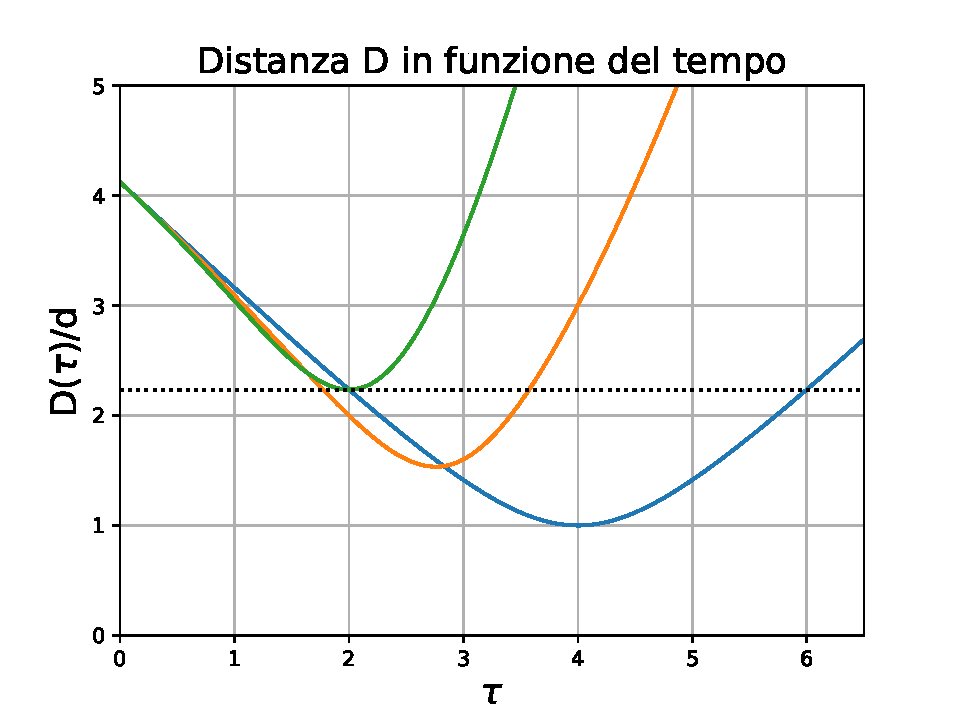
\includegraphics[scale=0.55]{distanza.pdf}
\caption{Funzione $D(\tau)$ per diversi $\alpha$. Il caso studiato nell'esercizio è rappresentato dalla linea verde. \label{fig:distanza} }
\end{figure}

\subsection{Lancio di un sasso da una collina \rstar\rstar}
Un ragazzo si trova in cima a una collina di pendenza $45^\circ$.
In un sistema di riferimento cartesiano posizionato alla 
base della collina la sua posizione è: $(0,h)$, mentre il profilo della collina è dato dalla retta:
%
\begin{equation*}
y=-x+h
\end{equation*} 
%
All'istante di tempo $t_0=0$ il ragazzo calcia
un sasso con velocità iniziale:
%
\begin{equation*}
\vec{v_0}=(v_0,0) \qquad v_0=15 \; \; \; \text{m/s}
\end{equation*} 
%
In che istante di tempo $t_1$ il sasso incontra di nuovo la collina?

\subsubsection*{Soluzione}
Il sasso si muove di moto uniformemente accelerato lungo $\hat{y}$, con accelerazione uguale a quella di gravità: $\vec{g}=-g \hat{y}$. Lungo $\hat{x}$ il moto invece è rettilineo uniforme. La legge oraria del sasso è quindi: 
%
\begin{gather*}
x(t)= v_0 t \\
y(t)= h - \frac{1}{2} g t^2
\end{gather*} 
%
Al tempo $t_1$ (nostra incognita), il sasso si trova di nuovo 
lungo il profilo della collina, per cui:
%
\begin{gather*}
y(t_1)=h- x(t_1) \quad \Rightarrow \quad h - \frac{1}{2} g t_1^2=h- v_0 t_1
\end{gather*} 
%
Ricaviamo quindi:
%
\begin{gather*}
 \frac{1}{2} g t_1^2= v_0 t_1  \quad \Rightarrow \quad t_1= \frac{2 v_0}{g}
\end{gather*} 
%
Inserendo i valori numerici si ottiene: 
%
\begin{gather*}
t_1= \frac{2\cdot 15 \text{  m/s}}{9.81 \text{  m/s}^2} \simeq 3.06 \text{  s}
\end{gather*} 
%

\subsection{Canestro! \rstar\rstar\rstar} 
Un pallone da basket è lanciato da un'altezza iniziale $h=2.40$ m con velocità iniziale $|\vec{v_0}|=12$ m/s. 
In un sistema di riferimento cartesiano, la posizione iniziale del pallone è quindi: $(0,h)$. L'angolo $\theta$ fra il vettore $\vec{v_0}$ e il versore $\hat{x}$ è $35^\circ$. Il giocatore che lancia il pallone riesce a centrare un canestro posizionato nel punto $(d,H)$ con $H=3.05$ m.  Qual è la distanza $d$ del giocatore dal canestro? Con quale angolo rispetto a $\hat{x}$ la palla entra nel canestro? Si supponga che il pallone sia approssimatile come un punto materiale. 

\subsubsection*{Soluzione}
Il vettore velocità iniziale è:
%
\begin{equation*}
\vec{v_0}=|v_0| \big(\cos(\theta), \sin(\theta)\big)
\end{equation*}
%
Il pallone da basket si muove di moto uniformemente accelerato lungo $\hat{y}$, con accelerazione uguale a quella di gravità: $\vec{g}=-g \hat{y}$. Lungo $\hat{x}$ il moto invece è rettilineo uniforme. La legge oraria del pallone è quindi: 
%
\begin{gather*}
x(t)= |v_0| t \cos(\theta)\\
y(t)= h + |v_0| t \sin(\theta) - \frac{1}{2} g t^2
\end{gather*} 
%
La traiettoria descritta dal pallone è una parabola. Possiamo ricavarne l'equazione, scrivendo $t=\frac{x(t)}{|v_0|  \cos(\theta)}$ e sostituendo nell'equazione per $y(t)$. Si ottiene così: 
%
\begin{gather*}
y= h + \frac{\sin(\theta)}{\cos(\theta)} x - \frac{1}{2}  \frac{g}{|v_0|^2  \cos^2(\theta)}x^2
\end{gather*} 
%
Sappiamo che la traiettoria passa per il canestro, cioè per il punto $(d,H)$. Allora:
%
\begin{gather*}
H= h + \frac{\sin(\theta)}{\cos(\theta)} d - \frac{1}{2}  \frac{g}{|v_0|^2  \cos^2(\theta)}d^2
\end{gather*} 
%
Questa è un'equazione di secondo grado per l'incognita $d$. Le due soluzioni sono:
%
\begin{gather*}
\frac{|v_0|^2 \cos^2(\theta)}{g}\bigg[+\frac{\sin(\theta)}{\cos(\theta)} \pm \sqrt{\frac{\sin^2(\theta)}{\cos^2(\theta)} - \frac{2 g (H-h)}{|v_0|^2  \cos^2(\theta)} }\bigg] 
\end{gather*} 
%
Ci sono due soluzioni, entrambe positive. Questo perché la parabola passa due volte per l'altezza $H$: a sinistra e a destra del massimo in altezza (Figura \ref{fig:71}). Sono entrambe soluzioni accettabili,  tuttavia sembra più verosimile che il giocatore di basket faccia canestro sfruttando la seconda soluzione, quella con il segno $+$. Si ottiene quindi:
%
\begin{gather*}
d=\frac{|v_0|^2 \cos^2(\theta)}{g}\bigg[+\frac{\sin(\theta)}{\cos(\theta)} + \sqrt{\frac{\sin^2(\theta)}{\cos^2(\theta)} - \frac{2 g (H-h)}{|v_0|^2  \cos^2(\theta)} }\bigg] 
\end{gather*} 
%

Sostituendo i numeri valori dati nel testo: $d \simeq 12.8$ m.
 \begin{figure}[!ht]
 \centering
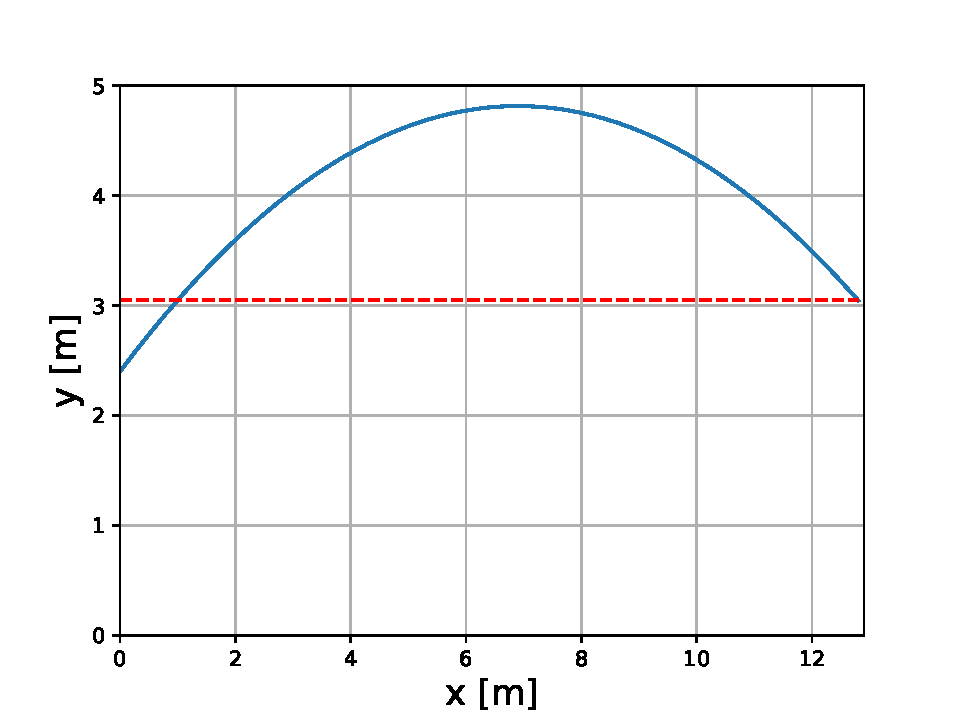
\includegraphics[scale=0.55]{71.pdf}
\caption{Traiettoria del pallone (linea continua). La linea tratteggiata indica l'altezza $H$ a cui si trova il canestro.\label{fig:71} }
\end{figure}
L'istante di tempo in cui il pallone entra nel canestro è: 
%
\begin{equation*}
t_f=\frac{d}{|v_0|  \cos(\theta)} \simeq 1.30 \text{  s}
\end{equation*}
%
La componente $x$ della velocità in questo momento è ovviamente $|v_0| \cos(\theta)$. La componente $y$ invece è:
%
\begin{equation*}
v_y(t_f)= |v_0|  \sin(\theta) - g t_f  \simeq - 5.88 \text{  m/s}
\end{equation*}
%
L'angolo con il quale il pallone entra nel canestro si trova 
considera
%
\begin{equation*}
\tan(\theta')=\frac{v_y(t_f)}{v_x(t_f)} \quad \Rightarrow \quad \theta' \simeq - 31^\circ
\end{equation*}
%

\subsection{Lancio doppio \rstar\rstar\rstar}
Un sasso $A$ è lasciato cadere da fermo dalla cima di un pozzo di altezza $h$ all'istante di tempo $t_0=0$. In quale istante di tempo $t_1$ esso tocca il fondo? A un certo istante di tempo $0<t_2<t_1$ viene lanciato 
un secondo sasso $B$, con velocità iniziale $\vec{v}=v \hat{y}$ (nel sistema di riferimento cartesiano in cui $\vec{g}=-g\hat{y}$ ). Come  dev'essere scelta la velocità $v$ affinché $B$ possa raggiungere $A$ prima che questo tocchi il fondo? Qual è il minimo valore del modulo di $v$ perché tale condizione sia realizzata? Calcolarne il valore numerico per $h=15$ m e $t_2=\frac{1}{2}t_1$. 

\subsubsection*{Soluzione}
La legge oraria del corpo $A$ è quella di un moto uniformemente accelerato lungo $\hat{y}$:
%
\begin{equation*}
y_A(t)=h- \frac{1}{2}g t^2
\end{equation*}
%
Quindi $A$ raggiunge il fondo all'istante $t_1= \sqrt{\frac{2h}{g}}$. 
La legge oraria di $B$ sarà:
%
\begin{equation*}
y_B(t)=h + v(t-t_2)- \frac{1}{2}g (t-t_2)^2 \qquad 0<t_2<\sqrt{\frac{2h}{g}}
\end{equation*}
%
La condizione che vogliamo che si verifichi è che $B$ raggiunga $A$ prima che questo tocchi il fondo. Questo significa che:
%
\begin{equation*}
y_B(\bar{t})=y_A(\bar{t}) 
\end{equation*}
%
per un qualche $\bar{t}$ appartenente all'intervallo $(t_2, t_1)$. La condizione diventa quindi:
%
\begin{equation*}
v(\bar{t}-t_2)- \frac{1}{2}g (\bar{t}-t_2)^2= - \frac{1}{2}g \bar{t}^2 \qquad t_2 < \bar{t} <t_1
\end{equation*}
%
Svolgendo il quadrato si ottiene:
%
\begin{equation*}
v(\bar{t}-t_2)- \frac{1}{2}g (-2\bar{t}t_2 + t_2^2)=0 \quad \Rightarrow \quad v=\frac{1}{2}g t_2\frac{t_2-2\bar{t}}{\bar{t}-t_2}
\end{equation*}
%
Occorre studiare $v$ come funzione di $\bar{t}$ nell'intervallo di interesse, ovvero $(t_2, t_1)$. In questo intervallo $v$ è sicuramente $<0$, perché  $\bar{t}>t_2$ e quindi $2\bar{t}>t_2$. Questo fatto ha un senso fisico intuitivo: il sasso $B$ deve essere lanciato con una certa velocità iniziale diretta verso il basso affinché possa raggiungere $A$, che ha già cominciato a cadere.  Per $\bar{t}\rightarrow t_2^+$ la funzione $v(\bar{t})$ diverge a $-\infty$. Per $\bar{t}\rightarrow t_1^-$ essa tende invece al valore :
%
\begin{equation*}
\frac{1}{2}g t_2\frac{t_2-2t_1}{t_1-t_2}
\end{equation*}
%
Nell'intervallo $(t_2, t_1)$ la funzione è crescente. In definitiva i valori
possibili di $v$ affinché $B$ incontri $A$ a un $\bar{t}$ minore di $t_2$ e maggiore di $t_1$ sono:
%
\begin{equation*}
-\infty < v < - \frac{1}{2}g t_2\frac{2t_1-t_2}{t_1-t_2}
\end{equation*}
%
Il minimo valore del modulo di $v$ è quindi $|v_{min}|=\frac{1}{2}g t_2\frac{2t_1-t_2}{t_1-t_2}$. Se, come indicato nel testo $t_2=\frac{1}{2}t_1$, allora: 
%
\begin{equation*}
|v_{min}|=\frac{3}{4}g t_1= \frac{3}{4}\sqrt{2hg}
\end{equation*}
%
Per $h=15$ m si ottiene $|v_{min}| \approx 12.8$ m/s. In Figura  \ref{fig:sasso} sono rappresentate le leggi orarie $y_A(t)$ e $y_B(t)$ in questo caso, per $v=-|v_{min}|$ (linea tratteggiata) e per $v=-2|v_{min}|$ (linea continua).

 \begin{figure}[!ht]
 \centering
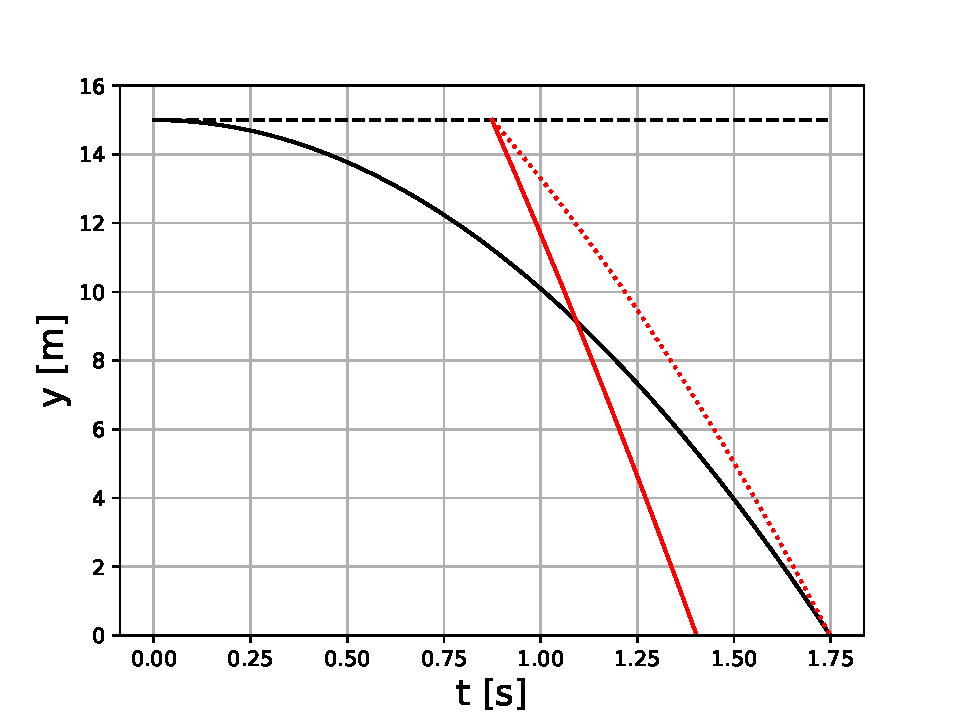
\includegraphics[scale=0.55]{sasso.pdf}
\caption{Legge oraria dei due sassi, per i valori numerici indicati nel testo e per due valori della velocità iniziale di $B$: $v=-|v_{min}|$ (linea tratteggiata) e $v=-2|v_{min}|$ (linea continua)}\label{fig:sasso} 
\end{figure}






\end{document}
